\documentclass{article}
\usepackage{graphicx} % Required for inserting images
\setlength{\parindent}{0pt}
\setlength{\parskip}{5pt}
\interfootnotelinepenalty=10000
\usepackage{microtype}
\usepackage{amsmath}
\usepackage{array}
\usepackage{hyperref}
\usepackage{tikz}
\sloppy

\title{Berkeley Energy and Resources Model for the California Economy Version 3.0 Technical Documentation}
\author{David Wells Roland Holst}
\date{November 2024}

\begin{document}

\maketitle


\newpage
\renewcommand{\abstractname}{\underline{\large Abstract}}
\begin{abstract}
The following document summarizes the structural characteristics of a dynamic forecasting model for the state of California, designed to support research into climate change, policy response, and their effects across this large and diverse state economy. The model integrates detailed treatment of sectoral production, employment, and demand with statewide assessment of environmental pollution and energy use over the next two decades. This model is currently under development and all technical details covered in this overview are subject to change. Thanks to Larry Goulder for helpful insights. All views expressed here are those of the author and should not be attributed to his affiliated institutions.
\end{abstract}

\newpage
\tableofcontents

\newpage
\section{Introduction}
This paper provides the complete technical specification of a computable general equilibrium model for the California economy, with detailed treatment of energy use and environmental pollution. Such a model can be used to support a broad spectrum of policy analysis, including energy policy and policy responses to climate change. The next section provides a brief overview of the main features of the model, which is followed by a detailed description of each block of the model.

\textbf{Production}

All sectors are assumed to operate under constant returns to scale and cost optimization. Production technology is modeled by a nesting of constant-elasticity-of-substitution (CES) functions. See Figure 1 for a schematic diagram of the nesting. The implementation of the model allows for all permissible special cases of the CES function, notably Leontief and Cobb-Douglas.

In each period, the supply of \textbf{primary} factors — capital, land, and labor — is usually predetermined\footnote{Capital supply is influenced by the current period’s level of investment.}. The model includes adjustment rigidities. An important feature is the distinction between old and new capital goods. In addition, capital is assumed to be partially mobile, reflecting differences in the marketability of capital goods across sectors\footnote{For simplicity, it is assumed that old capital goods supplied in second-hand markets and new capital goods are homogeneous. This formulation makes it possible to introduce downward rigidities in the adjustment of capital without increasing excessively the number of equilibrium prices to be determined by the model (see Fullerton, 1983).}.

Once the optimal combination of inputs is determined, sectoral output prices are calculated assuming competitive supply (zero-profit) conditions in all markets.

\textbf{Consumption and Closure Rule}

All income generated by economic activity is assumed to be distributed to consumers. Each representative consumer allocates optimally his/her disposable income among the different commodities and savings. The consumption/saving decision is completely static: saving is treated as a “good” and its amount is determined simultaneously with the demand for the other commodities, the price of saving being set arbitrarily equal to the average price of consumer goods\footnote{ The demand system is a version of the Extended Linear Expenditure System (ELES) which was first developed by Lluch (1973). The formulation of the ELES in this model is based on atemporal maximization — see Howe (1975). In this formulation, the marginal propensity to save out of supernumerary income is constant and independent of the rate of reproduction of capital.}.

The government collects income taxes, indirect taxes on intermediate inputs, outputs and consumer expenditures. The default closure of the model assumes that the government deficit/saving is exogenously specified\footnote{In the reference simulation, the real government fiscal balance converges (linearly) towards 0 by the final period of the simulation.}. The indirect tax schedule will shift to accommodate any changes in the balance between government revenues and government expenditures.

The current account surplus (deficit) is fixed in nominal terms. The counterpart of this imbalance is a net outflow (inflow) of capital, which is subtracted (added to) the domestic flow of savings. In each period, the model equates gross investment to net saving (equal to the sum of savings by households, the net budget position of the government and out of state capital inflows). This particular closure rule implies that investment is driven by saving.

\textbf{Trade}

Goods are assumed to be differentiated by region of origin, including goods from abroad and from the rest of the United States. In other words, goods classified in the same sector are different according to whether they are produced domestically or imported. This assumption is frequently known as the Armington assumption. The degree of substitutability, as well as the import penetration shares are allowed to vary across commodities and across agents. The model assumes a single Armington agent. This strong assumption implies that the propensity to import and the degree of substitutability between domestic and imported goods is uniform across economic agents. This assumption reduces tremendously the dimensionality of the model. In many cases this assumption is imposed by the data. A symmetric assumption is made on the export side where domestic producers are assumed to differentiate the domestic market and the export market. This is implemented using a Constant-Elasticity-of-Transformation (CET) production possibility frontier.

\textbf{Dynamic Features and Calibration}

The current version of the prototype has a simple recursive dynamic structure as agents are assumed to be myopic and to base their decisions on static expectations about prices and quantities. Dynamics in the model originate in three sources: i) accumulation of productive capital and labor growth; ii) shifts in production technology; and iii) the putty/semi-putty specification of technology.

\hspace{20pt}\textbf{(a) Capital accumulation}
 
In the aggregate, the basic capital accumulation function equates the current capital stock to the depreciated stock inherited from the previous period plus gross investment. However, at the sectoral level, the specific accumulation functions may differ because the demand for (old and new) capital can be less than the depreciated stock of old capital. In this case, the sector contracts over time by releasing old capital goods. Consequently, in each period, the new capital vintage available to expanding industries is equal to the sum of disinvested capital in contracting industries plus total savings generated by the economy, consistent with the closure rule of the model.

\hspace{20pt}\textbf{(b) The putty/semi-putty specification}

The substitution possibilities among production factors are assumed to be higher with the new than the old capital vintages — technology has a putty/semi-putty specification. Hence, when a shock to relative prices occurs (e.g. the imposition of an emissions tax), the demands for production factors adjust gradually to the long-run optimum because the substitution effects are delayed over time. The adjustment path depends on the values of the short-run elasticities of substitution and the replacement rate of capital. As the latter determines the pace at which new vintages are installed, the larger is the volume of new investment, the greater the possibility to achieve the long-run total amount of substitution among production factors.

\hspace{20pt}\textbf{(c) Dynamic calibration}

The model is calibrated on exogenous growth rates of population, labor force, and GDP. In the so-called Business-as-Usual (BaU) scenario, the dynamics are calibrated in each region by imposing the assumption of a balanced growth path. This implies that the ratio between labor and capital (in efficiency units) is held constant over time \footnote{This involves computing in each period a measure of Harrod-neutral technical progress in the capital-labor bundle as a residual. This is a standard calibration procedure in dynamic CGE modeling — see Ballard et. al. (1985).}. When alternative scenarios around the baseline are simulated, the technical efficiency parameter is held constant, and the growth of capital is endogenously determined by the saving/investment relation.

In the equations which follow, the following indices will be used extensively. Note that the time index generally be dropped from the equations.
{
\small

$i$	Production sectors. $j$ is an alias for $i$.\\
$nf$	Represents the non-fuel commodities.\\
$e$	Represents fuel commodities.\\
$l$	Represents the labor types.\\
$v$	Represents the capital vintages.\\
$h$	Represents the households.\\
$g$	Represents the government expenditure categories.\\
$f$	Represents the final demand expenditure categories (including $g$ as a subset).\\
$t$	Time index.\\

}

\section{Production}
Production is based on a nested structure of Constant Elasticity of Substitution (CES) functions. Each sector produces a gross output\footnote{Gross output is divided into two parts, one part produced with old capital, and the residual amount produced with new capital.}, $XP$, which given the assumption of constant returns to scale is undetermined by the producer. It will be determined by equilibrium conditions. The producer therefore minimizes costs subject to a production function which is of the CES type. At the first level, the producer chooses a mix of a value added aggregate, $VA$\footnote{The value added bundle also contains demand for energy, see below.}, and an intermediate demand aggregate, $ND$\footnote{Some models of this type assume a top level Leontief, i.e. a substitution elasticity of zero, in which case there is no substitution possibility between intermediate demand and value added. The GAMS implementation of the model can handle all of the special cases of the CES, i.e. Leontief and Cobb-Douglas.}.  In mathematical terms, this leads to the following formulation:
$$
\min PV\!A_i  V\!A_i + PN_i N\!D_i
$$
{\centering s.t. \par}

$$
X\!P_i = \left[a_{va,i}V\!A_{i}^{\rho_{i}^{p}}+a_{nd,i}N\!D_{i}^{\rho_{i}^p}\right]^{1/\rho_i^p}
$$
where $PVA$ is the aggregate price of value added, $PN$, is the price of the intermediate aggregate, $a_va$ and $a_nd$ are the CES share parameters, and $\rho$ is the CES exponent\footnote{The CES is described in greater detail in Appendix 1.}. The exponent is related to the CES elasticity, via the following relationship:
$$
p_i^p = \frac{\sigma_i^p-1}{\sigma_i^p}\Longleftrightarrow \sigma_i^p = \frac{1}{1-p_i^p} \ and \ \sigma_i^p \ge 0
$$
Note that in the model, the share parameters incorporate the substitution elasticity using the following relationships:
$$
\alpha_{va,i} = (a_{va,i})^{\sigma_i^p} \ and \ \alpha_{nd,i} = (\alpha_{nd,i})^{\sigma_i^p}
$$
Solving the minimization problem above, yields Equations (2.1.1) and (2.1.3) in Table 2.1. Because of the assumption of vintage capital, we are allowing the substitution elasticities to differ according to the vintage of the capital. Depending on the available data, and due to the importance of energy in terms of pollution, we separate energy demand from the rest of intermediate demand, and incorporate the demand for energy directly in the value added nest. Hence, the equations below are not specified in terms of a value added bundle, but a value added plus energy bundle. Equation (2.1.1) determines the volume of aggregate intermediate non-energy demand, by vintage, $ND$. Equation (2.1.2) determines the total demand for intermediate non-energy aggregate inputs (summed over vintages), $ND$. Equation (2.1.3) determines the level of the composite bundle of value added demand and energy, $KEL$. The CES dual price of $ND$, and $KEL$, $PXv$, is defined by Equation (2.1.4). Equation (2.1.5) determines the aggregate unit cost, $PX$, exclusive of an output subsidy/tax\footnote{The unit cost equation will be affected by production-specific emission taxes. Emission taxes are discussed in section 12.}. Finally, we allow the possibility of an output subsidy or tax, generating a wedge between the producer price and the output price, $PP$, yielding Equation (2.1.6). The production tax is multiplied by an adjustment factor which normally is fixed at unit value. However, it is possible to endogenize the average level of the production tax to achieve a predetermined fiscal target.

\newpage

\noindent\rule{\linewidth}{0.4pt}
\begin{center}
\begin{large}

{\centering Table 2.1: \textbf{Top Level Production Equations} \par}

\begin{tabular}{>{\raggedright}p{0.8\textwidth} l}

    $N\!D_j^v=\alpha^v_{nd,j}\left[\frac{P\!X_j^v}{P\!N_j}\right]^{\sigma^{p,v}_j} X\!Pv^v_j$ & (2.1.1) \\[10pt]
    $N\!D_j=\displaystyle \sum_{v} N\!Dv_j^v$ & (2.1.2) \\
    $K\!EL^v_j = \alpha^v_{kel,j}\left[\frac{PXv^v_j}{PKEL^v_j}\right]^{\sigma^{p,v}_j} X\!Pv^v_j$ & (2.1.3) \\[10pt]
    {\normalsize $PXv^v_j = \left[\alpha^v_{nd,j}PN_j^{1-{\sigma_j^{p,v}}}+\alpha^v_{va,j} PKEL_j^{v^{1-{\sigma_j^{p,v}}}}\right]^{1/({1-\sigma_j^{p,v}})}$} & (2.1.4) \\[10pt]
    $P\!X_j X\!P_j = \displaystyle \sum_v P\!Xv^v_j X\!Pv^v_j$ & (2.1.5) \\[10pt]
    $P\!P_j X\!P_j = P\!X_j(1+\delta^p\tau^p_j-\phi^p_j)X\!P_j$ & (2.1.6) \\[10pt]
\hline
\end{tabular}
\end{large}
\end{center}

The next level of the CES nest concerns on the one side aggregate intermediate demand, $N\!D$, and on the other side, the $K\!EL$ bundle. The split of $N\!D$ into intermediate demand is assumed to follow the Leontief specification, in other words a substitution elasticity of 0. (We also assume that the share coefficients are independent of the vintage.) The demand for non-fuel intermediate goods is determined by Equation (2.2.1). The intermediate demand coefficients are given by $a_{nf,j}$. The price of aggregate intermediate demand is given by adding up the unit price of intermediate demand. This is specified in Equation (2.2.2) in Table 2.2. Demand for each good is specified as a demand for the Armington composite (described in more detail below), an aggregation of a domestic good and an import good which are imperfect substitutes. Therefore, while there is no substitution of one intermediate good for another, there will be substitution between domestic demand and import demand depending on the relative prices. The price of the Armington good is given by $P\!A$.

At the same level, the $K\!EL$ bundle is split between labor and a capital-energy bundle, $K\!E$. It is assumed here as well, that the substitution possibilities between labor and the $K\!E$ bundle depend on the vintage of the capital. The optimization problem is similar to above, i.e. cost minimization subject to a CES aggregation function. If $AW$ is the aggregate sectoral wage rate, and $PKE$ is the price of the $K\!E$ bundle, aggregate labor demand, $AL$ and demand for the $K\!E$ bundle, are given by Equations (2.2.3) and (2.2.4). $\alpha_{l,i}$ and $\alpha_{ke,i}$ are the CES share parameters, and $\sigma^v$ is the CES elasticity of substitution. The price of $KEL$ bundle, $PKEL$, is determined by Equation (2.2.5), which is the CES dual price.

\newpage

\noindent\rule{\linewidth}{0.4pt}
\begin{center}
\begin{large}

{\centering Table 2.2: \textbf{Second Level CES Production Equations
} \par}

\begin{tabular}{>{\raggedright}p{0.8\textwidth} l}

$X\!Ap_{nf,j} = \displaystyle \sum_v a_{nf,j}N\!D^v_j$ & (2.2.1)\\
$PN_j = \displaystyle \sum_{nf} a_{nf,j}PA_{nf}$ & (2.2.2)\\
$AL^d_j = \displaystyle \sum_v \alpha^v_{l,j}\left[\frac{PKEL^v_j}{AW_j} \right]^{\sigma^{v,v}_j} KEL^v_j$ & (2.2.3)\\[12pt]
$K\!E^v_j = \alpha^v_{ke,j} \left[\frac{PKEL^v_j}{PKE^v_j} \right]^{\sigma^{v,v}_j} KEL^v_j$ & (2.2.4)\\[10pt]
{\normalsize $PKEL^v_j = \left[\alpha^v_{l,j}(AW_j)^{1-\sigma_j^{v,v}} + \alpha^v_{ke,j}(PKE^v_j)^{1-\sigma_j^{v,v}} \right]^{1/({1-\sigma_j^{v,v}})}$} & (2.2.5)\\[10pt]

\hline
\end{tabular}
\end{large}
\end{center}



The combined labor bundle is split into labor demand by type of labor, each with a specific wage rate, $W$\footnote{The current CALIFORNIA SAM includes 22 Standardized Occupational Code (SOC) labor categories. Depending on the level of labor disaggregation chosen, it might be appropriate to have a more detailed nesting structure for labor, rather than a single level nest.}. (Though labor markets are assumed to clear for each skill category, we allow for differential wage rates across sectors reflecting potential different institutional arrangements). Equation (2.3.1) determines labor demand by skill type in each sector, using a CES aggregation function. We allow for changes in labor efficiency which can be specified by both skill type and by sector. The dual price, or the average sectoral wage, $AW$, is defined by Equation (2.3.2).

\noindent\rule{\linewidth}{0.4pt}
\begin{center}
\begin{large}
{\centering Table 2.3: \textbf{Labor Demand
} \par}

\begin{tabular}{>{\raggedright}p{0.8\textwidth} l}

$L^d_{i,j} = \frac{\alpha^l_{lj}}{\lambda_{lj}} \left[\frac{\lambda_{lj}AW_j}{\Phi_{lj}W_l}\right]^{\sigma^l_j} AL^d_j$ & (2.3.1)\\[15pt]

$AW_j = \left[\displaystyle \sum_l \alpha^l_{lj} \left(\frac{\Phi_{lj}W_l}{\lambda_{lj}}\right)^{1-{\sigma^l_j}} \right]^{1/(1-{\sigma^l_j})}$ & (2.3.2)\\[15pt]

\hline
\end{tabular}
\end{large}
\end{center}

\newpage

The next table describes the disaggregation of the capital-energy bundle, $KE$, into its energy and capital-land components. Equation (2.4.1) determines the demand for aggregate energy. Equation (2.4.2) determines the demand for the capital-land bundle by vintage, $KT$, where $PKT$ is the price of the capital-land bundle. Equation (2.4.3) defines the dual price of the $KE$ bundle.

\noindent\rule{\linewidth}{0.4pt}
\begin{center}
\begin{large}

{\centering Table 2.4: \textbf{Capital-Land Bundle and Energy Bundle Demand
} \par}

\begin{tabular}{>{\raggedright}p{0.8\textwidth} l}

$Ev^v_j = \alpha^v_{e,j} \left[\frac {PKE^v_j} {PEv^v_j} \right]^{\sigma^{k,v}_j} KE^v_j$ & (2.4.1)\\

$KTv^{d,v}_j = \alpha^v_{kt,j} \left[\frac {PKE^v_j} {PKT^v_j} \right]^{\sigma^{k,v}_j} K\!E^v_j$ & (2.4.2)\\

{\normalsize$PKE^v_j = \left [\alpha^v_{e,j} \left(PEv^v_j \right)^{1-{\sigma^{k,v}_j}} + \alpha^v_{k,j} \left(PKT^v_j \right)^{1-{\sigma^{k,v}_j}}\right]^{1/(1-{\sigma^{k,v}_j})} $} & (2.4.3)\\[15pt]

\hline
\end{tabular}
\end{large}
\end{center}

The next level in the nest determines the demand for the capital and land factors. Equation (2.5.1) defines land demand by sector and vintage, $Tv$, where $PT$ is the price of land. Similarly, Equation (2.5.2) determines demand for capital by sector and vintage, $Kv$, where $R$ is the rental rate of capital. Note that the rental rate is both sector and vintage specific. Both equations incorporate technology shifters (which will be explained in the section on dynamics)\footnote{The current data for the CALIFORNIA model does not include land as a separate account, therefore the additional capital-land nest, though active, is irrelevant.}.  Equations (2.5.4) and (2.5.5) determine respectively aggregate sectoral land demand and capital demand.

\noindent\rule{\linewidth}{0.4pt}
\begin{center}
\begin{large}

{\centering Table 2.5: \textbf{Capital and Land Demand
} \par}

\begin{tabular}{>{\raggedright}p{0.8\textwidth} l}

$Tv^{d,v}_j = \frac {\alpha^v_{t,j}} {\lambda^v_{t,j}} \left   [\frac {\lambda^v_{t,j}PKT^v_j} {PT_j} \right]^{\sigma^{s,v}_j} KT^v_j$ & (2.5.1) \\

$Kv^{d,v}_j = \frac {\alpha^v_{k,j}} {\lambda^v_{k,j}} \left   [\frac {\lambda^v_{k,j}PKT^v_j} {R^v_j} \right]^{\sigma^{s,v}_j} KT^v_j$ & (2.5.2)\\[15pt]

$PKT^v_j = \left[\alpha^v_{t,j} \left(\frac{PT_j}{\lambda^v_{t,j}} \right)^{1-\sigma^{s,v}_j} + \alpha^v_{k,j} \left(\frac{R^v_j}{\lambda^v_{k,j}}\right)^{1-\sigma^{s,v}_j} \right]^{1/({1-\sigma^{s,v}_j})}$ & (2.5.3) \\[10pt]

$T^d_j = \displaystyle \sum_v Tv^{d,v}_j$ & (2.5.4) \\[10pt]

$K^d_j = \displaystyle \sum_v Kv^{d,v}_j$ & (2.5.5) \\[10pt]

\hline
\end{tabular}
\end{large}
\end{center}

The energy bundle determined by Equation (2.4.1) is further disaggregated by energy-type. The number of fuel types will depend on the available data. We let the index $e$ range over the number of fuel types (eventually the dimension of $e$ could even be 1). Equation (2.6.1) determines the demand for the different types of fuels. The $\lambda$ factor allows for energy efficiency improvement over time which can be sector specific, as well as vintage specific. Equation (2.6.2) determines the CES dual price, $PEv$, of the energy bundle.

\noindent\rule{\linewidth}{0.4pt}
\begin{center}
\begin{large}

{\centering Table 2.6: \textbf{Decomposition of the Energy Bundle} \par}

\begin{tabular}{>{\raggedright}p{0.8\textwidth} l}

$X\!Ap_{ej} = \displaystyle \sum_v \frac {\alpha^f_{e,j,v}} {\lambda^e_{jv}} \left[\frac {\lambda^e_{jv} PEv^v_j} {PA_e} \right]^{\sigma^f_{jv}} Ev^v_j$ & (2.6.1)\\[20pt]

$PEv^v_j = \left[\displaystyle \sum_e \alpha^f_{e,j,v} \left(\frac {P\!A_e} {\lambda^e_{jv}} \right)^{1-{\sigma^f_{jv}}} \right]^{1/(1-{\sigma^f_{jv}})}$ & (2.6.2)\\[15pt]

\hline
\end{tabular}
\end{large}
\end{center}

\section{Income Distribution}

Production generates income, both wage and non-wage, which is distributed in some form to three main institutions:  households, government, and financial institutions (both domestic and out of state).

Equation (3.1.1) determines gross operating surplus, $KY$. It is the sum across all vintages and all sectors of capital remuneration. Equation (3.1.2) defines company income, $CY$, it is equal to a share of gross operating surplus (the rest being distributed to households). Equation (3.1.3) determines corporate taxes, $Tax^c$. The base tax rate is given by the parameter $\kappa^c$. However, corporate taxes can be made endogenous (in order to meet a fiscal target, for example), in which case the adjustment parameter, $\delta^c$, becomes endogenous. Equation (3.1.4) defines retained earnings, i.e. corporate saving. Corporate saving is equal to a residual share of after-tax company income\footnote{In the reference simulation, both the private corporate saving rate and the household saving rate are adjusted (upwards), under the assumption that domestic saving, as a share of GDP, will increase in the future. The adjustments are based on rules of thumb, but could be made explicit in the model.}. The remaining amount of net company income is distributed to households.

\newpage

\noindent\rule{\linewidth}{0.4pt}
\begin{center}
\begin{large}
{\centering Table 3.1: \textbf{Corporate Earnings Equations} \par}

\begin{tabular}{>{\raggedright}p{0.8\textwidth} l}

$KY = \displaystyle \sum_v \sum_i R^v_i Kv^{d, v}_i$ & (3.1.1)\\[15pt]

$CY = \chi^k K\!Y$ & (3.1.2)\\[15pt]

$Tax^c = \delta^c\kappa^cCY$ & (3.1.3) \\[15pt]

$Sav^P_c = \left(1- \displaystyle \sum_h \phi^c_h \right)(1-\delta^c\kappa^c)CY$ & (3.1.4) \\[15pt]
\hline
\end{tabular}
\end{large}
\end{center}

Household income derives from two main sources, capital and labor income. Additionally, households receive transfers from the government. Equation (3.2.1) defines total labor income, $YL$ as the product of total labor demand and the wage rate.

Labor income is distributed to the households. Equation (3.2.2) defines total household income, $YH$. It is the sum of labor income, distributed capital income and net company income, income from land, and transfers from the government, $TR_g^h$. Capital, company, and land income are distributed to households using fixed shares. The adjustment factor $\delta^{HTr}$ on government transfers can be used as a fiscal instrument in order to achieve a specified target, similar to the adjustment factors on other taxes in the model. Household direct tax, $Tax^h$, is given by Equation (3.2.3), 

where $\kappa^h$ is the tax rate. The adjustment factor $\delta^{HTx}$ can be endogenous if the government saving/deficit is exogenous. In this case, the household tax schedules shifts in or out to achieve the net government balance. Otherwise, the household tax schedule is exogenous, and the factor stays at its initial value of 1. Finally Equation (3.2.4) defines household disposable income, $YD$. Disposable income is equal to total household income less taxes.

\section{Household Consumption and Savings}

Household disposable income is allocated to goods, services, labor, and savings using the \textit{Extended Linear Expenditure System} (ELES) specification\footnote{For references, see Lluch (1973) or Deaton and Muellbauer (1980).}. The consumer problem can be set up as follows:

\begin{center}

$\max U = \displaystyle \sum_{i=1}^n\mu_i\ln(C_i - \theta_i) + \mu_S\left(\frac{S}{cpi}\right)$\\
s.t. $\displaystyle \sum_{i=1}^n PC_iC_i + S = YD$\\
and $\sum_{i=1}^n\mu_i + \mu_s = 1$

\end{center}

where $U$ is the utility function, $C_i$ is consumption by commodity, $S$ is household saving, $PC$ is the vector of consumer prices, and $YD$ is disposable income. $\mu$ and $\theta$ are parameters which will be given an interpretation below. $S$ can be thought of as demand for a future bundle of consumer goods. For reasons of simplification, it is assumed that the saving bundle is evaluated using the consumer price index, $cpi$. Lluch provides a more detailed theoretical analysis of how savings enters the utility maximization problem.

Solving the above optimization problem leads to the following demand functions:
\begin{center}

$C_i = \theta_i + \frac{\mu_iY^*}{PC_i}$\\
$S = \mu_sY^* = YD - \displaystyle \sum_{i=1}^nPC_iC_i$\\
$Y^* = YD - \displaystyle \sum_{j=1}^nPC_j\theta_j$

\end{center}

Consumption is the sum of two parts, $\theta$, which is often called the \textit{subsistence minima} or \textit{floor consumption}, and a fraction of $Y^*$, which is often called the \textit{supernumerary income}. $Y^*$ is equal to disposable income less total expenditures on the subsistence minima.

Table 4.1 presents the equations of the consumer demand system. Equation (4.1.1) defines the consumer price vector (for goods and services), $PC$, it is the Armington price incorporating household specific indirect taxes and subsidies. Equation (4.1.2) defines supernumerary income, that is, disposable income less total expenditures on the subsistence minima. (The subsistence minima are adjusted each time period by the growth rate in population). Consumer demand for goods and services is given by Equation (4.1.3)\footnote{ As noted earlier, the $\mu$ parameters are adjusted in the reference simulation in order to increase the level of domestic saving.}. Household savings is determined as a residual and is given in Equation (4.1.4). Aggregate household saving is determined by Equation (4.1.5). Equation (4.1.6) defines the consumer price index.

\newpage

\noindent\rule{\linewidth}{0.4pt}
\begin{center}
\begin{large}
{\centering Table 4.1: \textbf{Household Consumption and Savings Equations} \par}

\begin{tabular}{>{\raggedright}p{0.8\textwidth} l}

$PC_{ih} = P\!A_i\left(1 + \tau^h_{ih}\right)\left(1 - \varphi^h_{ih}\right)$ & (4.1.1)\\[15pt]

$Y^*_h = Y\!D_h - Pop_h \displaystyle \sum_i PC_{ih} \theta_{ih}$ & (4.1.2)\\[15pt]

$XAc_{ih} = Pop_h\theta_{ih} + \mu_{ih}Y^*_h / PC_ih$ & (4.1.3) \\[15pt]

$HSav^p_h = Y]!D_h - \displaystyle \sum_i PC_{ih}XAc{ih}$ & (4.1.4) \\[15pt]

$S_h = \displaystyle \sum_h HSav^p_h$ & (4.1.5) \\[15pt]

$cpi_h = \frac{\displaystyle \sum_i PC_{ih}XAc_{ih}}{\displaystyle \sum_i PC_{ih, 0}XAc_{ih}}$ & (4.1.6) \\[20pt]

\hline
\end{tabular}
\end{large}
\end{center}

\section{Other Final Demands}

All other final demand accounts (except stock changes) are integrated into a single demand matrix component. In the most general version of the model, the final demand components are government current expenditures, government capital expenditures, private capital expenditures, trade and transport margins for domestic sales, and trade and transport margins for imports. All the final demand vectors are assumed to have fixed expenditure shares. The closure of the final demand accounts will be discussed below.

Equation (5.1.1) determines the composition of final demand for each of the final demand components. Demand for goods is determined as constant shares of the volume of total final demand, $TFD$. The index $f$ covers government current and capital expenditures, private capital expenditure, inventory change, and both domestic and import trade margin expenditures. Equation (5.1.2) determines the value of final demand expenditures, $TFDV$. Equation (5.1.3) determines the price of final demand expenditures inclusive of taxes and subsidies, $PFD$. Equation (5.1.4) determines the aggregate final demand price deflator for each type of final demand account, $PTFD$.

\newpage

\noindent\rule{\linewidth}{0.4pt}
\begin{center}
\begin{large}
{\centering Table 5.1: \textbf{Final Demand Expenditure Equations} \par}

\begin{tabular}{>{\raggedright}p{0.8\textwidth} l}

$X\!AFD^f_i = afd^f_iTFD_f$ & (5.1.1)\\[15pt]

$TFDV_f = \displaystyle \sum_i PFD^f_i X\!AFD^f_i$ & (5.1.2)\\[15pt]

$PFD^f_i = PAFD^f_i\left(1 + \tau^f_i\right)\left(1-\varphi^f_i\right)$ & (5.1.3)\\[15pt]

$PTFD_f = \displaystyle \sum_i afd^f_iPFD^f_i$ & (5.1.4) \\[20pt]

\hline
\end{tabular}
\end{large}
\end{center}

Government current expenditures include expenditures on goods and services. Government aggregate expenditures on goods and services are fixed in real terms. Total nominal government expenditures, $GExp$, is determined by Equation (5.2.1) in Table 5.2. There are several exogenous elements which enter this equation including transfers to households, $TR_g^h$. Note the potential adjustment factor attached to the household transfer variable. Also note that all domestic transfers are typically held fixed and are multiplied by a price index in order to insure the homogeneity of the model. Equation (5.2.2) defines the government expenditure deflator, $PG$. Finally, Equation (5.2.3) is simply an identity which equates aggregate real government expenditures to the variable $TFD$ (for the accounts indexed by $g$).

\noindent\rule{\linewidth}{0.4pt}
\begin{center}
\begin{large}
{\centering Table 5.2: \textbf{Current Government Expenditure Equations} \par}

\begin{tabular}{>{\raggedright}p{0.8\textwidth} l}

$GExp = \displaystyle\sum_g\sum_iPA_iXAFD^g_i$\\
\hspace{31pt} $+ \displaystyle\sum_g \left(FDIT_g - FDSubs_g\right) + P\displaystyle\sum_h\left(\delta^{HTr}TR^h_{g, h}\right)$ & (5.2.1)\\[15pt]

$PG_gTG_g = \displaystyle\sum_iPFD^g_iX\!AFD^g_i$ & (5.2.2)\\[15pt]

$TFD_g = TG_g$ & (5.2.3)\\[20pt]


\hline
\end{tabular}
\end{large}
\end{center}

\section{Government Revenues and Saving}

Government derives most of its revenues from direct corporate and household taxes, and indirect taxes. Subsidies are also provided which enter as negative revenues. Equations (6.1.1)-(6.1.4) in Table 6.1 list all the different indirect taxes paid by production activities, household consumption, final demand expenditures, and exports, respectively, $PIT_x$, $SIT_x$, $HIT_x$, $FDIT_x$, and $EIT_x$. Equation (6.1.5) describes the sum of all indirect taxes.

\noindent\rule{\linewidth}{0.4pt}
\begin{center}
\begin{large}
{\centering Table 6.1: \textbf{Indirect Tax Equations} \par}

\begin{tabular}{>{\raggedright}p{0.8\textwidth} l}

$PIT_x = \displaystyle\sum_i \left(\delta^p\tau^p_i-\varphi^p_i\right)PX_iXP_i$ & (6.1.1)\\

$HITx = \displaystyle \sum_h \sum_i PA_i\tau^h_{ih}XAc_{ih}$ & (6.1.2)\\

$FDITx_f = \displaystyle \sum_i PA_i \tau^f_i XAFD^f_i$ & (6.1.3)\\

$EITx = \displaystyle \sum_r \sum_i PEr_ir \tau^E_{ir} ESr_{ir}$ & (6.1.4)\\

$TlndTax = PITx + HITx + \displaystyle \sum_f FDITx_f + EITx$ & (6.1.5)\\[20pt]


\hline
\end{tabular}
\end{large}
\end{center}

Equations (6.2.1)-(6.2.3) in Table 6.2 define the level of subsidies for household consumption, other final demand expenditures, and exports, respectively, $HSubs$, $FDSubs$, and $ESubs$. Total subsidies is given by Equation (6.2.4).

\noindent\rule{\linewidth}{0.4pt}
\begin{center}
\begin{large}
{\centering Table 6.2: \textbf{Subsidy Equations} \par}

\begin{tabular}{>{\raggedright}p{0.8\textwidth} l}

$HSubs = \displaystyle \sum_h \sum_i PA_i \left(1 + \tau^h_{ih}\right)\varphi^h_{ih}XAc_{ih}$ & (6.2.1)\\

$FDSubs_f = \displaystyle \sum_i PA_i \left(1 + \tau^f_i\right)\varphi_i^fX\!AFD^f_i$ & (6.2.2)\\

$ESubs = \displaystyle \sum_r \sum_i PEr_ir \left(1 + \tau^E_{ir}\right)\varphi^E_{ir}ESr_{ir}$ & (6.2.3) \\

$TSubs = HSubs + \displaystyle \sum_f FDSubs_f + ESubs$ & (6.2.4) \\[20pt]

\hline
\end{tabular}
\end{large}
\end{center}

Table 6.3 defines fiscal closure for the government. Equation (6.3.1) describes total income from import tariffs, where $WPM$ are world prices, $\tau^m$ are tariffs, and $XMr$ represents import volumes. All the relevant import variables are doubly indexed since they represent variables by sector and region of origin. The exchange rate is used to convert world prices (e.g. in dollars) into local currency. There is an additional adjustment factor $\delta^{Tar}$ which allows the aggregate tariff rate to vary endogenously. Equation (6.3.2) identifies miscellaneous government revenue sources, these are all revenues less household direct taxes. Equation (6.3.3) provides total current government nominal revenues, $GRev$. Equation (6.3.4) and (6.3.5) define respectively the nominal and real level of government saving. Two government closure rules are implemented. Under the default rule, government saving is held fixed (typically at its base value), and one of the taxes (or government transfers to households) is allowed to adjust (uniformly) to achieve the government fiscal target. Under the second closure rule, all tax levels and transfers are fixed, and real government saving is endogenous. This latter rule can have significant consequences on the level of investment since investment is savings driven.

\noindent\rule{\linewidth}{0.4pt}
\begin{center}
\begin{large}
{\centering Table 6.3: \textbf{Government Revenues and Closure Equations} \par}

\begin{tabular}{>{\raggedright}p{0.8\textwidth} l}

$YTrade = ER\delta^{Tar} \displaystyle \sum_r \sum_i WPM_{ri}\tau^m_{ri}XMr_{ri}$ & (6.3.1)\\[15pt]

$MiscRev = Tax^c + TlndTax - TSubs + YTrade$ & (6.3.2)\\[15pt]

$GRev = MiscRev + Tax^h$ & (6.3.3)\\[15pt]

$S_g = GRev - GExp$ & (6.3.4)\\[15pt]

$RSg = S_r / P$ & (6.3.5)\\[20pt]

\hline
\end{tabular}
\end{large}
\end{center}

\section{Trade, Domestic Supply and Demand}

Similar to many trade CGE models, we have assumed that imported goods are not perfect substitutes for goods produced domestically\footnote{This is known as the Armington assumption — see Armington (1969).}. The degree of substitution will depend on the level of disaggregation of the commodities. For example, wheat is more substitutable as a commodity than grains, which in turn are more substitutable than a commodity called primary agricultural products. The Armington assumption reflects two stylized facts. Trade data shows the existence of two-way trade which is consistent with the Armington assumption. As well, and related, the Armington assumption leads to a model where perfect specialization, which is rarely observed, is avoided.

In this version of the model, we have adapted the CES functional specification for the Armington assumption. This has some undesirable properties which have been explored in more detail elsewhere\footnote{See for example Robinson et. al. (1992).}, but alternative formulations have proven to be deficient as well. The adoption of the \textit{Constant Elasticity of Transformation} (CET) specification for exports alleviates to some extent the deficiencies of the Armington CES specification. We also assume that there is only one domestic Armington agent, this is sometimes known as \textit{border-level} Armington specification. It is parsimonious in both data requirements and computational resources.

To allow for the existence of multiple trading partners, the model adopts a two-level CES nesting to represent the Armington specification (see Figure 2)\footnote{The current CALIFORNIA SAM has a single rest of the world account, i.e. an aggregate trading partner. The dual nesting is therefore redundant. However, both the data processing facility and the model retain the multiple trading partner specification in order to maintain flexibility for future data developments.}. At the top level, agents choose an optimal combination of the domestic good and an import aggregate which is determined by a set of relative prices and the degree of substitutability. Let $XA$ represent aggregate demand for an Armington composite, with the associated Armington price of $PA$. Each agent then minimizes the cost of obtaining the Armington composite, subject to an aggregation function. This can be formulated by:

\begin{center}

min \hspace{30pt} $PD \hspace{5pt} XD + PM \hspace{5pt} XM$\\[20pt]
s.t. \hspace{5pt} $XA = \left[a_dXD^\rho + a_mXM^\rho\right]^{1/\rho}$

\end{center}

where $XD$ is demand for the domestic good, $PD$ is the price of obtaining the domestic good, $XM$ is demand for the aggregate imported good, $PM$ is the aggregate import price, $a$ are the $CES$ share parameters, and $\rho$ is the $CES$ exponent. $\rho$ is related to the CES substitution elasticity via the following relation:

\begin{center}

$\rho = \frac{\sigma - 1}{\sigma} \Longleftrightarrow \sigma = \frac{1}{1-\rho}$

\end{center}

At the second level of the nest, agents choose the optimal choice of imports across regions, again as a function of the relative import prices and the degree of substitution across regions. Note that the import prices are region specific, as are the tariff rates. The second level nest also uses a CES aggregation function. The CES formulation implies that the substitution between any two pairs of importing partners is identical. Table 7.1 lists the solution of the optimization problem described above. Equation (7.1.1) determines domestic demand for the Armington aggregate across all agents of the economy, $XA$. Equations (7.1.2) and (7.1.3) determine respectively, the optimal demand for the domestic component of the Armington aggregate, $XD$, and aggregate import demand, $XM$. Equation (7.1.4) defines the price of the Armington bundle, $PA$, which is the CES dual price.

\noindent\rule{\linewidth}{0.4pt}
\begin{center}
\begin{large}
{\centering Table 7.1: \textbf{Top-level Armington Equations} \par}

\begin{tabular}{>{\raggedright}p{0.8\textwidth} l}

$X\!A_i = \displaystyle \sum_j X\!Ap_{ij} + \sum_h X\!Ac_{ih} + \sum_f X\!AFD_f$ & (7.1.1)\\[15pt]

$X\!D_i = \beta^d_i \left(\frac{PA_i}{PD_i}\right)^{\sigma^m_i} X\!A_i$ & (7.1.2)\\[15pt]

$X\!M_i = \beta^m_i \left(\frac{PA_i}{PM_i}\right)^{\sigma^m_i} XA_i$ & (7.1.3)\\[15pt]

$P\!A_i = \left[\beta^d_iPD_i^{1-{\sigma^m_i}}+\beta^m_iPM_i^{1-{\sigma^m_i}}\right]^{1/(1-{\sigma^m_i})}$ & (7.1.4)\\[20pt]


\hline
\end{tabular}
\end{large}
\end{center}

The equations in Table 7.2 describe the decomposition of the aggregate import bundle, $XM$ into its components, i.e. imports by region of origin. Each demand component will be a function of the price of the exporting partner, as well as partner-specific tariff rates. Equation (7.2.1) determines import volume by sector and region of origin, $XMr$, where $PMr$ is the partner specific import price, in domestic currency and inclusive of tariffs. Equation (7.2.2) defines the price of the aggregate import bundle, $PM$, which is the CES dual price. Finally, Equation (7.2.3) defines the domestic import price, $PMr$, which is equal to the import price of the trading partner, converted into local currency, and inclusive of the partner-specific tariff rate.

\noindent\rule{\linewidth}{0.4pt}
\begin{center}
\begin{large}
{\centering Table 7.2: \textbf{Second-level Armington Equations} \par}

\begin{tabular}{>{\raggedright}p{0.8\textwidth} l}

$X\!M_{ri} = \beta^r_{ri} \left(\frac{PM_i}{PMr_{ri}}\right)^{\sigma^w_i}X\!M_i$ & (7.2.1)\\[15pt]

$P\!M_i = \left[\displaystyle \sum_r \beta^r_{ri}\left(PMr_{ri}\right)^{1-{\sigma^w_i}}\right]^{1/(1-{\sigma^w_i})}$ & (7.2.2)\\[15pt]

$P\!Mr_{ri} = ER WPM_{ri}\left(1 + \tau^m_{ri}\right)$ & (7.2.3)\\[20pt]


\hline
\end{tabular}
\end{large}
\end{center}

Treatment of domestic production is symmetric to the treatment of domestic demand. Domestic producers are assumed to perceive the domestic market as different from the export market. The reason is similar:  a high level of aggregation. Further, export markets might be more difficult to penetrate, forcing perhaps different quality standards than those applicable for the domestic market. This formulation assumes a production possibilities frontier where each producer maximizes sales, subject to being on the frontier, and influenced by relative prices.

The optimization problem is formulated somewhat differently since the object of the local producer is to maximize sales, not to minimize costs. We therefore have:

\begin {center}

max $PD \hspace{5pt} XD + PE \hspace{5pt} ES$\\
s.t. $XP = \left[\gamma_d XD^\lambda + \gamma_e ES^\lambda \right]^{1/\lambda}$

\end{center}

where $XD$ is aggregate domestic sales of domestic production, $ES$ is out of state sales of domestic production (exports), with a producer export price of $PE$, $XP$ is aggregate domestic production with a producer price of $PP$, $\gamma$ are the CET share parameters, and $\lambda$ is the CET exponent. The CET exponent is related to the CET substitution elasticity, $\Lambda$ via the following relation:

\begin{center}

$\lambda = \frac{\Lambda + 1}{\Lambda} \Longleftrightarrow \Lambda = \frac{1}{\lambda - 1}$

\end{center}

Analogous to the Armington specification, producer supply decisions are assumed to be undertaken in two steps (see Figure 3). First, producers choose the optimal combination of domestic supply and aggregate export supply. Then, an additional step which optimizes export supply across trading partners. The top-level producer supply decisions, in reduced form, are given by Equations (7.3.1) and (7.3.2), where the share parameters are $\alpha^t$ and the CET substitution elasticity is $\sigma^t$.\footnote{Note the difference between the Armington CES and the CET.  First, the relation between the exponent and the substitution elasticity is different.  Second, the ratio of the prices and the share parameter in the reduced forms are inverted.  This is logical since the goal of the producer is to maximize revenues.  For example, an increase in the price of exports, relative to the composite aggregate price, will lead to an increase in export supply.} Equation (7.3.3) is the CET dual price function, which determines sectoral domestic output. If the CET elasticity is infinite, producers perceive no differentiation across markets, in which case both domestic and export goods are sold at the uniform producer price, $PP$, and output is simply the sum of domestic supply and export supply. (The formulas reflect an adjustment for stock building. Stock building is assumed to occur using only domestically produced goods, which are priced at the aggregate producer price, $PP$. Sectoral stock building is modeled as a fixed share of a volume of stock building, $StB$. This formulation implies that stock building is simply subtracted (added) from (to) total current output, $XP$.)

\newpage
\noindent\rule{\linewidth}{0.4pt}
\begin{center}
\begin{large}
{\centering Table 7.3: \textbf{Top-level CET Equations} \par}

\begin{equation}
    \begin{cases}
      XD_i = \alpha^t_{d, i} \left(\frac{PD_i}{PP_i} \right)^{\sigma^t_i} \left(XP_i - \alpha^{st}_i StB \right) \text{ if } \sigma^t_i < \infty\\
      PD_i = PP_i \text{ if } \sigma^t_i = \infty\\
    \end{cases}       
    \tag{7.3.1}
\end{equation}

\begin{equation}
    \begin{cases}
      ES_i = \alpha^t_{e, i} \left(\frac{PE_i}{PP_i} \right)^{\sigma^t_i} \left(XP_i - \alpha^{st}_i StB \right) \text{ if } \sigma^t_i < \infty\\
      PE_i = PP_i \text{ if } \sigma^t_i = \infty\\
    \end{cases}       
    \tag{7.3.2} 
\end{equation}

\begin{equation}
    \begin{cases}
      PP_i = \left[\alpha^t_{d, i} PD^{1 + \sigma^t_i}_i + \alpha^t_{e, i} PE^{1 + \sigma^t_i}_i \right]^{1/(1+ \sigma^t_i}) \text{ if } \sigma^t_i < \infty\\
      XP_i = XD_i +ES_i + \alpha^{st}_i StB \text{ if } \sigma^t_i = \infty\\
    \end{cases}       
    \tag{7.3.3}
\end{equation}

\end{large}
\end{center}
\noindent\rule{\linewidth}{0.4pt}

The second-level CET nest determines the optimal supply of exports to individual trading partners, $ESr$. Equation (7.4.1) defines export supply by region of destination. Equation (7.4.2) determines the aggregate export price, $PE$.

\noindent\rule{\linewidth}{0.4pt}
\begin{center}
\begin{large}
{\centering Table 7.4: \textbf{Second-level CET Equations} \par}


\begin{tabular}{>{\raggedright}p{0.8\textwidth} l}


$ESr_{ir} = \alpha^r_{ir}\left(\frac{PEr_{ir}}{PE_i}\right)^{\sigma^z_i}ES_i$ & (7.4.1)\\[15pt]

$PE_i = \left[\displaystyle\sum_r\alpha^r_{ir}\left(PEr_ir\right)^{1+{\sigma^z_i}}\right]^{1/{1+{\sigma^z_i}}}$ & (7.4.2)\\[20pt]

\hline
\end{tabular}
\end{large}
\end{center}

Table 7.5 presents the equations which determine export demand by the regional trading partners, and the export market equilibrium condition. Equation (7.5.1) defines export demand by trading partner, $ED$. If the exporting country has some market power, it will face a downward sloping demand curve. This is implemented using a constant elasticity function, with the elasticity given by $\sigma^e$. Export demand will also be influenced by the price of competing exports. This is reflected in the variable WPINDEX, which is exogenous since it is assumed the domestic economy does not influence export prices of its trading partners. (Changes in the WPINDEX could show the impacts of exogenous changes in the terms-of-trade). Under the small-country assumption the export demand elasticity is infinite, and the exporting country faces a flat demand curve, i.e. the export price is fixed (in dollar terms). Equation (7.5.2) converts the domestic export producer price into the domestic export price inclusive of taxes and subsidies (however, it is still in local currency). Equation (7.5.4) defines the export market equilibrium, i.e. the equality between domestic export supply and out of state demand.

\noindent\rule{\linewidth}{0.4pt}
\begin{center}
\begin{large}
{\centering Table 7.5: \textbf{Export Demand and Market Equilibrium} \par}


\begin{equation}
    \begin{cases}
      $$ED_{ir} = \alpha^e_{ir} \left(\frac{ER WPINDEX_{ir}}{WPE_{ir}} \right)^{\sigma^e_{ir}}$$ \text{ if } $$\sigma^e_{ir} < \infty$$\\
      $$WPE_{ir} = ER WPINDEX_{ir}$$ \text{ if } $$\sigma^e_{ir} = \infty$$\\
    \end{cases}       
    \tag{7.5.1}
\end{equation}

\begin{tabular}{>{\raggedright}p{0.8\textwidth} l}

$WPE_{ir} = \left(1 + \tau^E_{ir} \right) \left(1 - \varphi^e_{ir} \right) PEr_{ir}$ & (7.5.2)\\[15pt]

$ESr_{ir} = ED_{ir}$ & (7.5.3)\\[15pt]

\hline

\end{tabular}
\end{large}
\end{center}

\section{Equilibrium Conditions}

The first factor market equilibrium condition concerns labor. Labor demand, by skill type is generated by production decisions. In terms of supply, the model implements a simple labor supply curve, where labor supply is a function of the real wage. Equation (8.1.1) defines the labor supply curve. If the supply elasticity is less than infinity, labor supply is a function of the equilibrium real wage rate. In the extreme case where the elasticity is zero, labor is fully employed and fixed. If the elasticity is infinite, the real wage is fixed and there is no constraint on labor supply. This may be an appropriate assumption in cases where the level of unemployment is relatively high. Equation (8.1.2) determines equilibrium on the labor market. If the labor supply curve is not flat, it determines the equilibrium wage rate. If the labor supply curve is flat, it sets labor supply identically equal to aggregate labor demand. Labor by skill type is assumed to be perfectly mobile across sectors, therefore Equation (8.1.2) determines the uniform wage by skill type. Because the model allows for wages to vary across sectors, the uniform wage is actually the aggregate wage which varies uniformly across sectors for each skill type, and the relative wages across sectors are held fixed at their base levels.

\noindent\rule{\linewidth}{0.4pt}
\begin{center}
\begin{large}
{\centering Table 8.1: \textbf{Equilibrium Conditions for the Labor Market} \par}

\begin{equation}
    \begin{cases}
      $$L^s_l = a_l \left(\frac{W_l}{P} \right)^{\omega_l}$$ \text{ if } $$\omega_l < \infty$$\\
      $$W_l = P \overline{W}_l$$ \text{ if } $$\omega_l = \infty$$\\
    \end{cases}       
    \tag{8.1.1}
\end{equation}

\begin{tabular}{>{\raggedright}p{0.8\textwidth} l}

$\displaystyle \sum_i L^d_{l, i} = L^s_l$ & (8.1.2)\\[15pt]

\hline
\end{tabular}
\end{large}
\end{center}

Land market demand, similar to demand for labor and capital, is generated by the production sector. Land supply is modeled using the CET specification. If the elasticity is infinite, land is perfectly mobile across sectors. If the elasticity is zero, land is fixed and sector-specific. Between these two extreme values, land is partially mobile and sectoral supply will reflect the relative rate-of-return of land across sectors. Equations (8.2.1)-(8.2.3) reflect either situation (finite or infinite). In the case of a finite CET elasticity, Equation (8.2.1) determines the aggregate price of land, \textit{PLand}, which is the CET dual price. \textit{TLand} is aggregate land supply which is exogenous. Equation (8.2.2) determines sectoral supply of land, $T^s$, and Equation (8.2.3) is the equilibrium condition which determines the sector-specific land price, $PT$. In the case of infinite elasticity, Equation (8.2.1) determines the aggregate (uniform) price of land through an equilibrium condition which equates total land supply, \textit{TLand}, to aggregate land demand. Equation (8.2.2) trivially sets the sectoral land price equal to the economy-wide land price, and Equation (8.2.3) equates sectoral supply to sectoral demand.

\noindent\rule{\linewidth}{0.4pt}
\begin{center}
\begin{large}
{\centering Table 8.2: \textbf{Land Supply and Market Equilibrium} \par}

\begin{equation}
    \begin{cases}
      $$PLand = \left[\displaystyle \sum_i \alpha^{ts}_i PT^{1/(1+\omega^s)} \right]$$ \text{ if } $$\omega^s < \infty$$\\
      $$TLand = \displaystyle \sum_i T^d_i$$ \text{ if } $$\omega^s = \infty$$\\
    \end{cases}       
    \tag{8.2.1}
\end{equation}

\begin{equation}
    \begin{cases}
      $$T^s_i = \alpha^{ts}_i \left(\frac{PT_i}{PLand} \right)^{\omega^s} TLand$$ \text{ if } $$\omega^s < \infty$$\\
      $$PT_i = Pland$$ \text{ if } $$\omega^s = \infty$$\\
    \end{cases}       
    \tag{8.2.2}
\end{equation}

\begin{tabular}{>{\raggedright}p{0.8\textwidth} l}

$T^s_i = T^d_i$ & (8.2.3)\\[15pt]

\hline
\end{tabular}
\end{large}
\end{center}

\section{Determination of Vintage Output and Capital Market Equilibrium}

The model is set up to run in either comparative static mode or recursive dynamic mode. Capital market equilibrium is different in the two cases, and each will be described separately.

\textit{Comparative Static Capital Market Equilibrium}

In comparative static mode, there is no distinction made between old and new capital. Each sector determines demand for a single aggregate capital good. On the supply side, the model implements a CET supply allocation function (similar to land above). There is a single “capitalist” who owns all the capital in the economy, and supplies it to the different sectors based on each sector’s rate of return. Capital mobility across sectors is determined by the “capitalist’s” CET substitution elasticity. The substitution elasticity is allowed to vary from 0 to infinity. If the elasticity is 0, there is no capital mobility. This is an adequate description of a short term scenario. In the polar case, the substitution elasticity is infinite and there is perfect capital mobility. An intermediate value would allow for partial capital mobility.

The equations in Table 9.1 determine the equilibrium conditions for the capital market in comparative static mode. Equation (9.1.1) determines the aggregate rental rate. If there is partial capital mobility, the aggregate rental rate is the CET dual price of the sector specific rates of return. If there is perfect capital mobility, the aggregate rental rate is determined by an equilibrium condition which equates aggregate capital demand to total capital supply. Equation (9.1.2) determines either sectoral capital supply, or the sectoral rental rate. If capital is partially mobile, sectoral capital supply is determined by the CET first order condition, i.e. sectoral capital supply is a function of each sector's relative rate of return. If capital is perfectly mobile, the equivalent condition identically sets the sectoral rate of return to the economy-wide rate of return. Finally, Equation (9.1.3) determines the sectoral rate of return in the case of partial capital mobility. Under perfect capital mobility, it trivially equates capital supply to capital demand.

\noindent\rule{\linewidth}{0.4pt}
\begin{center}
\begin{large}
{\centering Table 9.1: \textbf{Capital Market Equilibrium in Comparative Static} \par}

\begin{equation}
    \begin{cases}
      $$TR = \left[\displaystyle \sum_i \alpha^s_i R^{1 + \Lambda}_i \right]^{1/(1+\Lambda}$$ \text{ if } $$\Lambda < \infty$$\\
      $$TK^s = \displaystyle \sum_i K^d_i$$ \text{ if } $$\Lambda = \infty$$\\
    \end{cases}       
    \tag{9.1.1}
\end{equation}

\begin{equation}
    \begin{cases}
      $$K^s_i = \alpha^s_i \left(\frac{R_i}{TR} \right)^\Lambda TK^s$$ \text{ if } $$\Lambda < \infty$$\\
      $$R_i = TR$$ \text{ if } $$\Lambda = \infty$$\\
    \end{cases}       
    \tag{9.1.2}
\end{equation}

\begin{tabular}{>{\raggedright}p{0.8\textwidth} l}

$K^s_i = K^d_i$ & \hfill (9.1.3)\\[20pt]

\hline
\end{tabular}
\end{large}
\end{center}


Recursive-Dynamic Capital Market Equilibrium
Sectoral output is essentially determined by aggregate demand for domestic output, see Equation (7.3.3). (In the simplest case, with no market differentiation, output is equal to the sum of domestic demand for domestic output, plus export demand, i.e. $XP = XD+ED$.) The producer decides the optimal way to divide production of total output across vintages. At first, the producer will use all the capital installed at the beginning of the capital, this is the depreciated installed capital from the previous period. If demand exceeds what can be produced with the old capital, the producer will demand new capital. If demand is lower than the output which can be produced with the old capital, the producer will disinvest some of the installed capital.
Equation (9.2.1) provides the capital/output ratio for old capital, $\chi$ (note that $Kv^{d,Old}$ reflects the optimal capital demand for old capital by the producer). Once the capital/output ratio is determined, it is easy to determine the optimal output using old capital. Equation (9.2.2) determines this quantity, $XPv^{Old}$, where an upper bound is given by total output. If the producer owns too much old capital, i.e. the desired output exceeds total demand, the producer will disinvest the difference between the initial capital stock and the capital stock which will produce the desired demand. Equation (9.2.3) determines output produced with new capital as a residual.


\noindent\rule{\linewidth}{0.4pt}

\begin{center}
\begin{large}


{\centering Table 9.2: \textbf{Determination of Vintage Output} \par}

\begin{tabular}{>{\raggedright}p{0.8\textwidth} l}

$\chi^{Old}_i = \frac{Kv^{d,Old}_i}{KPv^{Old}_i}$ & (9.2.1) \\[20pt]

$XPv^{Old}_i = min\left(K^s_{i,0} / \chi^{Old}_i, XP_i \right)$ & (9.2.2) \\[15pt]

$XPv^{New}_i = XP_i - XPv^{New}_i$ & (9.2.3) \\[20pt]

\hline
\end{tabular}
\end{large}
\end{center}

If a sector is in decline, i.e. it has too much installed capital given its demand, it will disinvest. The capital supply curve is a simple constant elasticity function of the relative rental rates. The higher the rental rate on old capital, the higher the supply of old capital. The formula which is used is:

\begin{center}

$K^{s,Old}_i = K^s_{i, o}\left[\frac{R^{Old}_{i, t}/R^{New}_{i, t}}{R^{Old}_{i, t-1}/R^{New}_{i, t-1}}\right]^{\eta^k_i}$

\end{center}

where $\eta^k$ is the disinvestment elasticity. Another way to think of this is to subtract the two capital numbers, i.e.

\begin{center}

$K^s_{i, 0} - K^{s, Old}_i = K^s_{i, o}\left[1- \left(\frac{R^{Old}_{i, t}/R^{New}_{i, t}}{R^{Old}_{i, t-1}/R^{New}_{i, t-1}}\right)^{\eta^k_i}\right]$

\end{center}

This represents the supply of disinvested capital, which increases as the relative rental rate of old capital decreases. At the limit, when the rental rates are equalized, there is no disinvested capital. At equilibrium, demand for old capital (in each declining sector), must equal supply of old capital. We can therefore invert the first equation to determine the rental rate on old capital, assuming the sector is in decline and supply equals demand. Equation (9.3.1) determines the relative rental rate on old capital for sectors in decline, i.e. it is the ratio of the old rental rate to the new rental rate. It is bounded above by 1, because the rental rate on old capital in declining sectors is not allowed to exceed the rental rate on new capital.
Equation (9.3.2) determines the rental rate on mobile capital. Mobile capital is the sum of new capital, disinvested capital, and installed capital in expanding sectors. It is not necessary to subtract immobile capital from each side of the capital equilibrium condition, i.e. the rental rate on mobile capital can be determined from the aggregate capital equilibrium condition. Equation (9.3.3) is an identity setting the rental rate on new capital equal to the rental rate on mobile capital. Equation (9.3.4) determines the rental rate of old capital. If a sector is disinvesting, the rental rate on old capital is essentially determined by Equation (9.3.1). If a sector is expanding, then $RR$ is equal to 1, and therefore the rental rate on old capital in expanding sectors will be equal to the rental rate of new capital.

\noindent\rule{\linewidth}{0.4pt}

\begin{center}
\begin{large}
{\centering Table 9.3: \textbf{Capital Market Equilibrium} \par}


\begin{tabular}{>{\raggedright}p{0.8\textwidth} l}


$RR_{i, t}= min\left(1, RR_{i, t-1}\left(\frac{Kv^{d, v}_i)}{K^s_{i, 0}}\right)^{1/{\eta^k_i}}\right)$ & (9.3.1) \\[15pt]

$\displaystyle \sum_i K^d_i = K^s$ & (9.3.2) \\[15pt]

$R^{New}_i = TR$ & (9.3.3) \\[15pt]

$R^{Old}_i = TR\hspace{5pt}RR_i$ & (9.3.4) \\[20pt]

\hline
\end{tabular}
\end{large}
\end{center}

\section{Macro Closure}

Government closure was discussed above, current government savings are determined either endogenously with fixed tax rates, or exogenously, with one of the tax adjustment factors endogenous.
Equation (10.1.1) is the ubiquitous savings equals investment equation. In Equation (10.1.1), $TFDV_{zp}$ is the value of private investment expenditures, whose value must equal total resources allocated to the private investment sector:  retained corporate earning, $Sav^P_c$, total household savings, $S_{hr}$, government savings, $S_{gr}$, the sum across regions of out of state capital flows, $S_{fr}$, and net of stock building expenditures.
The last closure rule concerns the balance of payments. First, we make the small country assumption for imports, i.e. local consumption of imports will not affect the border price of imports, $WPM$. Equation (10.1.2) is the overall balance of payments equation. The value of imports, at world (border) prices, must equal the value of exports, at border prices (i.e. inclusive of export taxes and subsidies) plus net transfers and factor payments, and plus net capital inflows. The balance of payments constraint is dropped from the model due to Walras’ Law
The final equations of the model, Equations (10.1.3)-(10.1.5) are used to calculate the domestic price index which is used to inflate real domestic transfers. Note that real GDP is measured in efficiency units. The numéraire of the model is the exchange rate.

\noindent\rule{\linewidth}{0.4pt}
\begin{center}
\begin{large}
{\centering Table 10.1: \textbf{Closure Equations} \par}
\end{large}
\begin{small}
\begin{tabular}{>{\raggedright}p{0.8\textwidth} l}

$TFDV_{zp} = Sav^P_c + S_h + ER\displaystyle\sum_r S_{fr}+S_g - \sum_i \alpha^{st}_iPP_iStB$ & (10.1.1) \\[15pt]

$\displaystyle\sum_r\sum_iWPM_{ri}XMr_{ri} = \sum_r\sum_i \frac{WPE_{ir}}{ER}ESr_{ir}+\sum_r S_{fr}$ & (10.1.2) \\[15pt]

$GDPVA = \displaystyle \sum_l W_l \sum_i \Phi_{li} L^d_{li} + \sum_i \sum_v PT_iTv^{d, v}_i + \sum_i \sum_v R^v_i Kv^{d, v}_i$ & (10.1.3) \\[15pt]




{\tiny $RGDP = \displaystyle \sum_l W_{l, 0} \sum_i \Phi_{li} \lambda^l_{li} L^d_{li} + \sum_i \sum_v PT_{i, 0} \lambda^v_{t, i} Tv^{d, v}_i + \sum_i \sum_v R^v_{i, 0} \lambda^v_{k, i} Kv^{d, v}_i$} & (10.1.4) \\[15pt]


$P = \frac{GDPVA}{RGDP}$ & (10.1.5) \\[20pt]

\hline
\end{tabular}
\end{small}
\end{center}

\section{Dynamics}

\textit{\textbf{Predetermined Variables}}

The first table presents the variables which are pre-determined, i.e. they do not depend on any contemporaneous endogenous variables. Equation (11.1.1) determines the labor supply shift factor which is equal to the previous period’s labor supply shift factor multiplied by an exogenously specified labor supply growth rate. (All dynamic equations reflect the fact that the time steps may not be of equal size. The growth rates are always given as per cent per annum increases.) Equation (11.1.2) provides a similar equation for population. The population and labor growth rates are allowed to differ. Government (real) expenditures and the transfers between government and households grow at the rate of growth of GDP. This latter growth rate is exogenously specified (for the BaU scenario). Equations (11.1.3)-(11.1.4) provide the relevant formulas. Users can input their own exogenous assumptions about these variables. Equation (11.1.5) determines the amount of installed capital at the beginning of the period. If a sector is expanding, this will equal the amount of old capital in the sector at the end of the period. If a sector is declining, the amount of old capital at the end of the period will be less than the initial installed capital. The depreciation rate is exogenous.

\noindent\rule{\linewidth}{0.4pt}
\begin{center}
\begin{large}
{\centering Table 11.1: \textbf{Predetermined Variables} \par}


\begin{tabular}{>{\raggedright}p{0.8\textwidth} l}

$\alpha_{i, t} = \left(1 + \gamma^l\right)^n a_{l, t-n}$ & (11.1.1) \\[15pt]

$Pop_t = \left(1 + \gamma^p\right)^n Pop_{t-n}$ & (11.1.2) \\[15pt]

$TG_t = \left(1 + \gamma^y\right)^n TG_{t-n}$ & (11.1.3) \\[15pt]

$TR^h_{g, t} = \left(1 + \gamma^y\right)^n TR^h_{g, t-n}$ & (11.1.4) \\[15pt]

$K^s_{i, 0, t} = \left(1 - \delta\right)^n K^d_{i, t-n}$ & (11.1.5) \\[20pt]

\hline
\end{tabular}
\end{large}
\end{center}

\textbf{\textit{Capital Stock}}
The motion equation for the aggregate capital stock is given by the following 1-step formula:

\begin{center}

$K_t = (1-\delta)K_{t-1}+l_{t-1}$

\end{center}

where $K$ is the aggregate capital stock, $\delta$ is the annual rate of depreciation, $I_{t-1}$ is the level of real investment in the previous period. Using mathematical induction, we can deduce the multi-period transition equation:

\begin{center}

$K_t = (1-\delta)[(1-\delta)K_{t-2}+I_{t-2}]+I_{t-1}$\\
.\\[-0.5em] % Adjust the vertical space as needed
.\\[-0.5em]
.\\
$K_t = (1-\delta)^nK_{t-n} + \displaystyle \sum^n_{j=1}(1-\delta)^{j-1}I_{t-j}$

\end{center}

If the step size is greater than 1, the model does not calculate the intermediate values for the path of real investment. The investment path is estimated using a simple linear growth model, i.e.

\begin{center}

$I_j = (1+\gamma^i)I_{j-1}$

\end{center}

where

\begin{center}

$\gamma^i = \left(\frac{I_t}{I_{t-n}}\right)^{1/n}-1$

\end{center}

Note that the formula for the investment growth depends on the contemporaneous level of real investment. This explains why the current capital stock is not predetermined. If real investment increases (e.g. because out of state transfers increase), this will have some effect on the current capital stock via its influence on the estimated growth rate of real investment. Inserting the formula for the estimated real investment stream in the capital stock equation, we derive:

\begin{center}

$K_t = (1 - \delta)^n K_{t-n} + \displaystyle \sum^n_{j=1} (1-\delta)^{j-1} (1 + \gamma^i)^{n-j} I_{t-n}$

\end{center}

A little bit of algebra, yields Equation (11.2.1) for the aggregate capital stock. Equation (11.2.2) defines the annualized growth rate of real investment which is used to calculate the aggregate capital stock. Equation (11.2.3) determines the level of normalized capital. There are two indices of capital stock. The first index is the normalized level of capital stock. This index is called normalized because it is the level of capital stock in each sector which yields a rental rate of 1. The second index is the actual level of the capital stock, given in base year prices. The latter variable is only used in two equations. It is used to determine the depreciation allowance, and it is used to update the level of the capital stock in Equation (11.2.1) (because it is in the same units as the level of real investment)\footnote{The following numerical example may clarify the issue. Assume the value of the capital stock is 100. Assume, as well, that capital remuneration is 10. Capital remuneration is simply $rK$ where $r$ is the rental rate and $K$ the demand for capital. In this example, $rK$ is equal to 10, which implies a rental rate of 0.1. The model assumes a normalization rule such that the rental rate is 1, and normalizes the capital data to be consistent with the normalization rule. In other words, the normalized capital demand is 10, and it is really an index of capital volume. The non-normalized level of capital is used only in the accumulation function and in determining the value of the depreciation allowance. All other capital stock equations use the normalized value of capital.}.

\newpage
\noindent\rule{\linewidth}{0.4pt}
\begin{center}
\begin{large}
{\centering Table 11.2: \textbf{Aggregate Capital Stock} \par}


\begin{tabular}{>{\raggedright}p{0.8\textwidth} l}


$K_t = (1-\delta)^n K_{t-n} + \frac{(1+\gamma^i)^n - (1-\delta)^n}{\gamma^i + \delta} I_{t-n}$ & (11.2.1) \\[15pt]

$\gamma^i = \left(\frac{I_t}{I_{t-n}}\right)^{1/n} - 1$ & (11.2.2) \\[15pt]

$K^s_t = \frac{K^s_{t-n}}{K_{t-n}}K_t$ & (11.2.3) \\[20pt]

\hline
\end{tabular}
\end{large}
\end{center}

\textbf{\textit{Productivity}}
Productivity enters the value-added bundle — labor, land, and capital — as separate efficiency parameters for the three factors, differentiated by sector and by vintage. In the current version of the model, and for lack of better information, the labor efficiency factor (and the energy efficiency factor) are exogenous. In defining the reference simulation, the growth path of real GDP is pre-specified, and a single economy-wide efficiency factor for land and capital is determined endogenously. In subsequent simulations, i.e. with dynamic policy shocks, the capital and land efficiency factors are exogenous, and the growth rate of real GDP is endogenous. 
Equation (11.3.1) defines the growth rate of real GDP. In defining the reference simulation, both lagged real GDP and the growth rate $\gamma^Y$ are exogenous, therefore the equation is used to determine the common efficiency factor for land and capital. In subsequent simulations, Equation (11.3.1) determines $\gamma^y$, i.e. the growth rate of real GDP. Equations (11.3.2) and (11.3.3) determine respectively the efficiency factors for capital and land. Both are set to the economy-wide efficiency parameter determined by Equation (11.3.1), however, the model allows for a partition of sectors, where the index $i'$ indexes a subset of all the sectors. It is assumed that the sectors not indexed by $i'$ have no efficiency improvement in land-capital. Equation (11.3.4) determines the common capital-labor efficiency growth factor, which is stored in a file for subsequent simulations. There are alternative methods for specifying and implementing the reference scenario.

\newpage
\noindent\rule{\linewidth}{0.4pt}
\begin{center}
\begin{large}
{\centering Table 11.3: \textbf{Capital-Land Efficiency} \par}

\begin{tabular}{>{\raggedright}p{0.8\textwidth} l}


$RGDP_t = (1 + \gamma^y)^n RGDP_{t-n}$ & (11.3.1) \\[15pt]

$\lambda^v_{t,i'} = \lambda_{kt}$ & (11.3.2) \\[15pt]

$\lambda^v_{t,i'} = \lambda_{kt}$ & (11.3.3) \\[15pt]

$\lambda_{kt,t} = (1 + \gamma^{kt}_t)^n \lambda_{kt, t-n}$ & (11.3.4)\\[20pt]

\hline
\end{tabular}
\end{large}
\end{center}

\textbf{\textit{Vintage Re-Calibration}}
At the beginning of each new period, the parameters of the production structure need to be modified to reflect the changing composition of capital. As a new period begins, what was new capital gets added to old capital, i.e. the new Old capital has a different composition from the previous Old capital. A simple rule is used to re-calibrate the production structure: the parameters are calibrated such that they can reproduce the previous period’s output using the aggregate capital of the previous period, but with the Old elasticities. (The parameters of the New production structure are not modified.) The relevant formulas are not reproduced here but can be found in the GAMS code.


\section{Emissions}

Emissions data for the BEAR model have been assembled from a variety of state, Federal, and independent sources. In the current version of the model, thirteen types of individual and composite emissions are represented (Table 12.1). The primary data relevant to AB32 come from California's own emissions inventory, cataloged from various sources by the California Energy Commission.

\newpage
\begin{center}
\begin{large}
{\centering Table 12.1: \textbf{Emission Types} \par}


\begin{tabular}{l r}
\hline\\[5pt]


Air Pollutants\\
1. \hspace{10pt} Suspended particulates & PART\\
2. \hspace{10pt} Sulfur Dioxide (SO\textsubscript{2}) & SO2\\
3. \hspace{10pt} Nitrogen Dioxide (NO\textsubscript{2} & NO2\\
4. \hspace{10pt} Volatile organic compounds & VOC\\
5. \hspace{10pt} Carbon monoxide (CO) & CO\\
6. \hspace{10pt} Toxic air index & TOXAIR\\
7. \hspace{10pt} Biological air index & BIOAIR\\[15pt]

Water Pollutants\\
8. \hspace{10pt} Biochemical oxygen demand & BOD\\
9. \hspace{10pt} Total suspended solids & TSS\\
10. \hspace{10pt} Toxic water index & TOXWAT\\
11. \hspace{10pt} Biological water index & BIOWAT\\[15pt]

Land Pollutants\\
12. \hspace{10pt} Toxic land index & TOXSOL\\
13. \hspace{10pt} Biological land index & BIOSOL\\[20pt]

\hline
\end{tabular}
\end{large}
\end{center}

To model the emission generation process, we incorporate emissions production into sectoral production functions. In much work of this kind, emission data have been directly associated with the volume of output. This has several consequences. First, the only way to reduce emissions, with a given technology, is to reduce output. This can lead to unpleasant messages for policy makers. A second consequence is that it ignores important sources of pollution outside the production side of the economy, namely household consumption. In an attempt to ameliorate these shortcomings, the pollution data for California has been regressed on a small subset of inputs of the state's corresponding input-output table. Using this econometric approach, we have shown elsewhere that the level of emissions can be explained by a very small subset of inputs (primarily fuels and chemicals)\footnote{See Dessus et. al. (1994).}. Incorporating these inputs into value added then allows production in the model to substitute away from polluting inputs. We assume that household emissions are affected by the relative prices of pollution-intensive goods and services in consumption.

Equation (12.2.1) defines the total level of emissions for each pollutant $p$. The bulk of the pollution is assigned to final demand for goods and services, represented by the bracketed second term in the expression. The first term in Equation (12.2.1) represents what we call process pollution. It is the residual amount of pollution in production which is not explained by the consumption of inputs. In the estimation procedure, a process dummy proved to be significant in certain sectors. If an emission fee (or tax) is exogenous, they are specified in physical units, i.e. dollars per ton. Equation (12.2.2) converts this into a nominal amount.

The equations in Table 12.3 describe how the model is modified to account for pollution fee/tax incidence. The underlying fee/tax can be generated in one of two ways, either be specified exogenously (in which case it is multiplied by a price index to preserve the homogeneity of the model), generated endogenously be specifying a constraint on the level of emission. The latter case, for example, corresponds to a Cap and Trade program, and Equation (12.2.1) is used to define the pollution constraint, while the fee/tax (e.g. permit price) generated by the constraint is the shadow price of Equation (12.2.1), and Equation (12.2.2) is not active.

\noindent\rule{\linewidth}{0.4pt}
\begin{center}
\begin{small}
{\centering \large{Table 12.2: \textbf{Emission Levels}} \par}

\begin{tabular}{>{\raggedright}p{0.8\textwidth} l}

$E_p = \displaystyle \sum_i \nu^p_iXP_i + \sum_i \pi^p_i \left(\sum_j XAp_{ij} + \sum_h XAc_{ih} \sum_f XAFD^i_f \right)$ & (12.2.1) \\[15pt]

{\large$\tau_{Poll} = P \bar{\tau}_{Poll}$} & (12.2.2) \\[20pt]

\hline
\end{tabular}
\end{small}
\end{center}

For accounting purposes, the tax can be implemented as an excise tax, i.e. it is implemented as a tax per unit of emission in currency units, i.e. \$x per ton of emission. It is converted to a price wedge on the consumption of the commodity (as opposed to a tax on the emission), using the commodity specific emission coefficient. For example, in Equation (2.1.5'), the tax adds an additional price wedge between the unit cost of production exclusive of the pollution tax, and the final unit cost of production. Let production equal 100 (million dollars for example), and let the amount of pollution be equal to 1 ton of emission per 10 million dollars of output. Then the total emission in this case is 10 tons. If the fee/tax is equal to \$25 per ton of emission, the total tax bill for this sector is \$250. In the formula below, $\nu$ is equal to 0.1 (tons per million dollars of output), $XP$ is equal to 100 (million dollars), and $t_p$ is equal to \$25. The consumption based pollution tax is added to the Armington price, see Equation (7.1.4'). However, the Armington decomposition occurs using basic prices, therefore, the taxes are removed from the Armington price in the decomposition formulae, see Equations (7.1.2') and (7.1.3'). Equation (6.3.3') determines the modification to the government revenue equation.

\newpage
\noindent\rule{\linewidth}{0.4pt}
\begin{center}
\begin{large}
{\centering Table 12.3: \textbf{Emission Price Wedges} \par}

\begin{tabular}{>{\raggedright}p{0.8\textwidth} l}


$PX_jXP_j = \displaystyle \sum_v PXv^v_j XPv^v_j + \sum_p \nu^p_j XP_j \tau_{Poll}$ & (2.1.5') \\[15pt]

{\small$PA_i = \left[\beta^d_i PD^{1-{\sigma^m_i}}_i + \beta^m_i PM^{1 - {\sigma^m_i}}_i \right]^{1/(1-{\sigma^m_i})} + \displaystyle \sum_p \pi^p_i \tau_{Poll}$} & (7.1.4') \\[15pt]

$XD_i = \beta^d_i \left(\frac{PA_i - \displaystyle \sum_p \pi^p_i \tau_{Poll}}{PD_i} \right)^{\sigma^m_i} XA_i$ & (7.1.2') \\[15pt]

$XM_i = \beta^m_i \left(\frac{PA_i - \displaystyle \sum_p \pi^p_i \tau_{Poll}}{PM_i} \right)^{\sigma^m_i} XA_i$ & (7.1.3') \\[15pt]

$GRev = Miscrev + Tax^h + \displaystyle \sum_p \tau_{Poll} E_p$ & (6.3.3') \\[20pt]

\hline
\end{tabular}
\end{large}
\end{center}

\section{Dealing with Uncertainty - Stochastic Variational Analysis}

Economic policy is subject to a broad range of systematic uncertainties, during development, implementation, and beyond. In other human endeavors, uncertainty is also pervasive, but in some fields it has been effectively managed with statistical methods. In engineering generally and the electric power sector in particular, reliability analysis is critical to hedge against risks of uncertain specification, design, materials, and operating conditions. Indeed, there is a large literature on most components of modern energy systems, including generation technologies, transmission systems, etc\footnote{ See e.g. Mazumdar and co-authors, Snyder and Stremel (1990), Scully et al (1992), and others cited below.}. 

Likewise, financial markets manage extensive risk patterns with statistical methods, including the same Monte Carlo methods popularized by engineers. Simpler “stress test” models of stochastic net present value inform most large project investments, but the spirit of these approaches is the same. In economic forecasting, there is also a long Monte Carlo tradition of “sensitivity analysis”, mainly intended to overcome uncertainty in estimates of behavioral parameters\footnote{ See, e.g. Thissen (1998) for a survey, as well as Abler et al (1999), Belgodere et al (2011). In energy modeling, see also Borenstein and co-authors.}.

What has been largely missing is an efficient methodology for what might be termed “policy reliability analysis,” a tractable empirical framework that can quantify the potential costs of uncertainty facing economic decision makers. It is somewhat surprising that most forecasters still report point estimates for events in the distant future, using scenario analysis to compare seemingly deterministic differences in outcomes of qualitatively different policies or states of nature. In reality, it is only possible to anticipate an interval of outcomes from any action, hopefully with a corresponding degree of confidence. This approach might be more responsible for those who forecast, but it offers an important degree of robustness against very real risks faced by those who enact and implement policies.

Until now, Monte Carlo methods would have been the tool of choice for this kind of policy research. Unfortunately, the statistical properties of this (randomized drawing approach) have many limitations, including resource requirements and instability in some applications. Fortunately, a new generation of numerical integration methods from physics and applied mathematics promises to greatly improve both the efficiency and accuracy of stochastic methods, and we apply this in the present report.

\textbf{\textit{Gaussian Quadrature}}

As an alternative to Monte Carlo methods, a numerical method called Gaussian Quadrature can approximate the distribution functions needed to do mean and variance analysis against parametric uncertainty. The basic goal is to approximate mean and variance, defined by integrals of the distribution of CGE model parameters or exogenous variable values a.

Generally, the Gaussian quadrature approach yields nodes $x_i$ and weights $\omega_i$ that can approximate a corresponding integral.

\begin{center}

$\int^b_a f(x)\omega(x)dx \approx \displaystyle \sum^L_{i=1} \omega_i f(x_i).$

\end{center}

In the present case, we seek nodes $a_i$ and weights $g_i$ to approximate means and variances of variables forecast by the CGE model, i.e.

\begin{center}

$m = \int_A h(a)dG = \int_A h(a)g(a)da \approx \displaystyle \sum^L_{i=1} g_i h(a_i) = \tilde{m}$,\\[20pt]

$\upsilon = \int_A (h(a) - m)^2 dG = \int_a (h(a) - m)^2 g(a)da \approx \displaystyle \sum^L_{i=1} g_i(h(a_i)-\tilde{m})^2 = \tilde{\upsilon},$

\end{center}

Based on this perspective, Hermeling et al (2013) develop a version of Gauss quadrature based on \textit{orthogonal polynomials}. This extends a traditional Gauss quadrature algorithm previously used in economics (cf. Arndt 1996 and DeVuyst and Preckel 1997), using functional forms better adapted to underlying standard probability distributions and thus realizing substantial gains in computational efficiency/accuracy. We summarize their approach here as it will be applied to the BEAR model.

Define orthogonality by the integral scalar product

\begin{center}

$(f_1, f_2)_g = \int_A f_1(a) f_2(a) dG = \int_A f_1(a) f_2(a) g(a) da$

\end{center}

A standard result of functional analysis (cf. Rudin 1976, ch. 7, p. 159) guarantees that any continuous (e.g. density) function, can be approximately with arbitrary accuracy by orthogonal polynomials whose roots define a finite set of approximations of approximation points. The best-known examples of orthogonal polynomials suited to modeling probability densities are Legendre, Tchebychev, Laguerre and Hermite, summarized below:

\begin{footnotesize}
\begin{tabular}{c|c|c|l} 
Name & $g(x)$ & {$[a, b]$} & Definition \\
\hline \hline Legendre & 1 & {$[-1,1]$} & $P_{k}(x)=\frac{(-1)^{k}}{2^{k} k!} \frac{d^{k}}{d x^{k}}\left[\left(1-x^{2}\right)^{k}\right]$ \\

Tschebyscheff & $\left(1-x^{2}\right)^{-\frac{1}{2}}$ & {$[-1,1]$} & $T_{k}(x)=\cos \left(k \cos ^{-1}(x)\right)$ \\

Laguerre & $\exp (-x)$ & {$[0, \infty)$} & $L_{k}(x)=\frac{\exp (x)}{k!} \frac{d^{k}}{d x^{k}}\left(x^{k} \exp (-x)\right)$ \\

Hermite & $\exp \left(-x^{2}\right)$ & $(-\infty, \infty)$ & $H_{k}(x)=(-1)^{k} \exp \left(x^{2}\right) \frac{d^{k}}{d x^{k}}\left(\exp \left(-x^{2}\right)\right)$
\end{tabular}
\end{footnotesize}

In practice, then, for a given density function g(a), we calculate the zeros $a_1, ..., a_k$ of the corresponding orthogonal polynomial of degree k. Calculating the weights $g_1, ..., g_k$ from a suitable system of linear equations, we obtain an integration formula that integrates polynomials up to degree 2k-1 exactly, using weights from the density function g(a).
For higher dimensional variational analysis (n>1), joint density integration can be approximated by using analogous polynomials and product rules, combining one-dimensional nodes and weights

\begin{center}

$\int^{\bar{a}^1}_{\underbar{a}^1} ... \int^{\bar{a}^d}_{\underbar{a}^d} f(a^1, ..., a^d)g^1(a^1) ... g^d(a^d)da^d...da^1$\\
$\approx \displaystyle \sum^n_{i_1 = 1} ... \sum^n_{i_d = 1} g^1_{i_1} ... g^d_{i_d} f(a^1_{i_1},..., a^d_{i_d})$

\end{center}

The additivity of nodes makes this approach dramatically more efficient than Monte Carlo multivariate analysis. With the former, function evaluations increase multiplicatively, while with MC they increase exponentially. 

\section*{Appendix 1 - The CES/CET Functions}
\addcontentsline{toc}{section}{Appendix 1 - The CES/CET Functions}

Because of the frequent use of the constant elasticity of substitution (CES) function, this appendix will develop some of the properties of the CES, including some of its special cases. The CES function can be formulated as a cost minimization problem, subject to a technology constraint:

\begin{center}

$min \displaystyle \sum_i P_iX_i$\\
subject to\\
$V = \left[\displaystyle \sum_i a_i (\lambda_i X_i)^\rho \right]^{1/\rho}$

\end{center}

where $V$ is the aggregate volume (of production, for example), $X$ are the individual components (“inputs”) of the production function, $P$ are the corresponding prices, and $a$ and $\lambda$ are technological parameters. $a$ are most often called the share parameters. $\lambda$ are technology shifters. The parameter $\rho$ is the CES exponent, which is related to the CES elasticity of substitution, which will be defined below.
A bit of algebra produces the following derived demand for the inputs, assuming $V$ and the prices are fixed:

where we define the following relationships:

$$
\begin{gathered}
\rho=\frac{\sigma-1}{\sigma} \Leftrightarrow \sigma=\frac{1}{1-\rho} \text { and } \sigma \geq 0 \\
\alpha_{i}=a_{i}^{\sigma}
\end{gathered}
$$
(1)\\[15pt]
and

$$
P=\left[\sum_{i} \alpha_{i} \lambda_{i}^{\sigma-1} P_{i}^{1-\sigma}\right]^{1 /(1-\sigma)}
$$
(2)\\[15pt]
$P$ is called the CES dual price, it is the aggregate price of the CES components. The parameter $\sigma$, is called the substitution elasticity. This term comes from the following relationship which is easy to derive from Equation (1):

$$
\frac{\partial\left(X_{i} / X_{j}\right)}{\partial\left(P_{i} / P_{j}\right)} \frac{\left(P_{i} / P_{j}\right)}{\left(X_{i} / X_{j}\right)}=-\sigma
$$

In other words, the elasticity of substitution between two inputs, with respect to their relative prices, is constant. (Note, we are assuming that the substitution elasticity is a positive number). For example, if the price of input increases by 10 percent with respect to input $j$, the ratio of input $i$ to input $j$ will decrease by (around) $\sigma$ times 10 percent.
The Leontief and Cobb-Douglas functions are special cases of the CES function. In the case of the Leontief function, the substitution elasticity is zero, in other words, there is no substitution between inputs, no matter what the input prices are. Equations (1) and (2) become:


$$X_{i}=\frac{\alpha_{i} V}{\lambda_{i}}$$
(1')
$$P=\sum_{i} \alpha_{i} \frac{P_{i}}{\lambda_{i}}$$
(2')

The aggregate price is the weighted sum of the input prices. The Cobb-Douglas function is for the special case when $\sigma$ is equal to one. It should be clear from Equation (2) that this case needs special handling. The following equations provide the relevant equations for the Cobb-Douglas:

$$
X_{i}=\alpha_{i} \frac{P}{P_{i}} V
$$
(1")
$$
P=A^{-1} \prod_{i}\left(\frac{P_{i}}{\alpha_{i} \lambda_{i}}\right)^{\alpha_{i}}
$$
(2")\\
where the production function is given by:
$$
V=A \prod_{i}\left(\lambda_{i} X_{i}\right)^{\alpha_{i}}
$$
and
$$
\sum_{i} \alpha_{i}=1
$$

Note that in Equation (1") the value share is constant, and does not depend directly on technology change.

\textit{Calibration}

Typically, the base data set along with a given substitution elasticity are used to calibrate the CES share parameters. Equation (1) can be inverted to yield:
$$
\alpha_{i}=\frac{X_{i}}{V}\left(\frac{P_{i}}{P}\right)^{\sigma}
$$
assuming the technology shifters have unit value in the base year. Moreover, the base year prices are often normalized to 1 , simplifying the above expression to a true value share. Let's take the Armington assumption for example. Assume aggregate imports are 20, domestic demand for domestic production is 80, and prices are normalized to 1 . The Armington aggregate volume is 100 , and the respective share parameters are 0.2 and 0.8 . (Note that the model always uses the share parameters represented by $a$, not the share parameters represented by $a$. This saves on compute time since the $a$ parameters never appear explicitly in any equation, whereas $a$ raised to the power of the substitution elasticity, i.e. a, occurs frequently.)
With less detail, the following describes the relevant formulas for the CET function which is similar to the CES specification.
$$
\begin{array}{cc}
\max & \sum_{i} P_{i} X_{i} \\
\text { s.t. } & V=\left[\sum_{i} g_{i} X_{i}^{\lambda}\right]^{1 / \lambda}
\end{array}
$$
where $V$ is the aggregate volume (e.g. aggregate supply), $X$ are the relevant components (sector-specific supply), $P$ are the corresponding prices, $g$ are the CET share parameters, and $\lambda$ is the CET exponent. The CET exponent is related to the CET substitution elasticity, $\Lambda$ via the following relation:
$$
\lambda=\frac{\Lambda+1}{\Lambda} \Leftrightarrow \Lambda=\frac{1}{\lambda-1}
$$

Solution of this maximization problem leads to the following first order conditions
$$
\begin{gathered}
X_{i}=\gamma_{i}\left(\frac{P_{i}}{P}\right)^{\Lambda} V \\
P=\left[\sum_{i} \gamma_{i} P_{i}^{1+\Lambda}\right]^{1 /(1+\Lambda)}
\end{gathered}
$$
where the Y parameters are related to the primal share parameters, $g$, by the following formula:
$$
\gamma_{i}=g_{i}^{-\Lambda} \Leftrightarrow g_{i}=\left(\frac{1}{\gamma_{i}}\right)^{1 / \Lambda}
$$

\newpage
\section*{Figures}
\begin{center}

Figure 1:\textbf{ Production Nesting}


\begin{scriptsize}
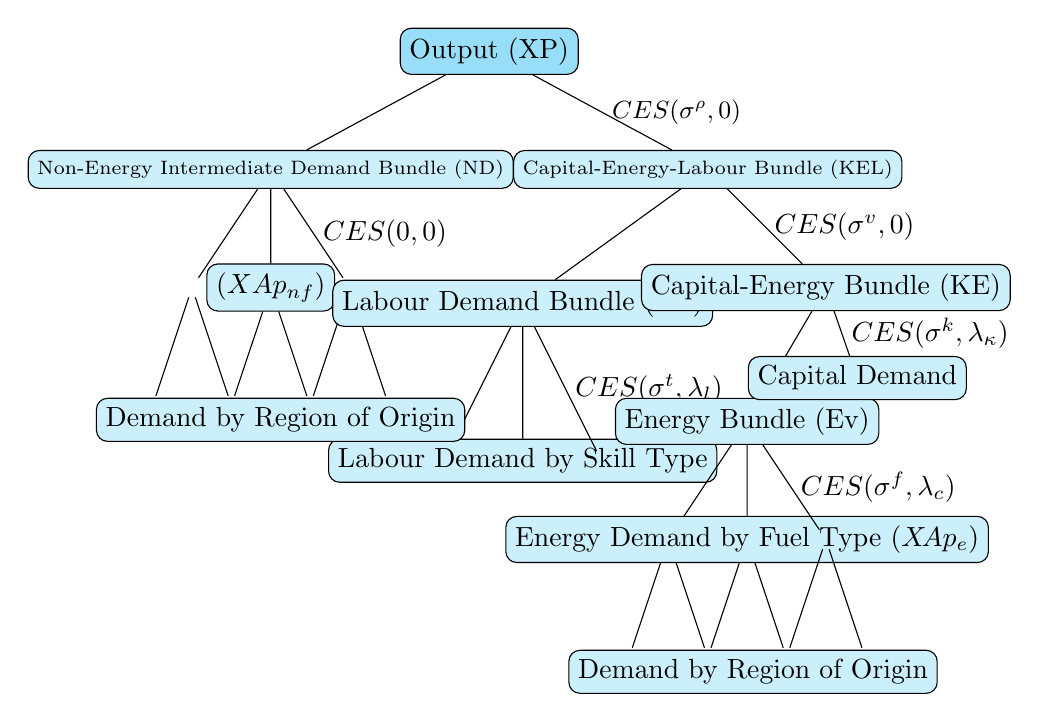
\begin{tikzpicture}

\tikzset{
    level 1/.style={sibling distance=5.55cm},
    level 2/.style={sibling distance=1cm}
}
\node[draw, fill=cyan!40, rounded corners] {\normalsize Output (XP)}
    child {node[draw, fill=cyan!20, rounded corners] {\scriptsize Non-Energy Intermediate Demand Bundle (ND)}
        child{node { }
            child{node { }}
            child{node { }}
        }
        child{node[draw, fill=cyan!20, rounded corners] {$(XAp_{nf})$}
            child{node { }}
            child{node { }}
        }
        child{node { }
            child{node { }}
            child{node { }}
            edge from parent node[right] {$CES(0, 0)$}
        }
    } 
    child {node[draw, fill=cyan!20, rounded corners] {\scriptsize Capital-Energy-Labour Bundle (KEL)}
        child{node[draw, fill=cyan!20, rounded corners] [shift={(-1.85cm, -0.2cm)}]{Labour Demand Bundle (AL)}
            child{node [shift={(0, -0.5cm)}] { }}
            child{node[draw, fill=cyan!20, rounded corners] [shift={(0, -0.5cm)}] {Labour Demand by Skill Type}}
            child{node [shift={(0, -0.5cm)}] { } edge from parent node[right] {$CES(\sigma^t, \lambda_l)$}}     
        }
        child{node[draw, fill=cyan!20, rounded corners] [shift={(1cm, 0)}] {Capital-Energy Bundle (KE)} 
            child{node[draw, fill=cyan!20, rounded corners] [shift={(-0.5cm, -0.2cm)}] {Energy Bundle (Ev)}
                child{node { }
                    child{node { }}
                    child{node { }}
                }
                child{node[draw, fill=cyan!20, rounded corners] {Energy Demand by Fuel Type ($X\!Ap_e$)}
                    child{node { }}
                    child{node { }}
                }
                child{node { }
                    child{node { }}
                    child{node{ }}
                    edge from parent node[right] {$CES(\sigma^f, \lambda_c)$}
                }
            }
            child{node[draw, fill=cyan!20, rounded corners] [shift={(-0.1cm, 0.35cm)}] {Capital Demand} edge from parent node[right] {$CES(\sigma^k, \lambda_\kappa)$}}
            edge from parent node[right] {$CES(\sigma^v, 0)$}
        }
        edge from parent node[right] {\small$CES(\sigma^\rho, 0)$}
    };
    \path (-2.65,-4.4) node[below][draw, fill=cyan!20, rounded corners] {Demand by Region of Origin};
    \path (3.35,-7.6) node[below][draw, fill=cyan!20, rounded corners] {Demand by Region of Origin};
\end{tikzpicture}
\end{scriptsize}
\end{center}

\textit{Notes:}
\begin{footnotesize}

1.\hspace{10pt} Each nest represents a different CES bundle. The first argument in the CES function represents the substitution of elasticity. The elasticity may take the value zero. Because of the putty/semi-putty specification, the nesting is replicated for each type of capital, i.e. old and new. The values of the substitution elasticity will generally differ depending on the capital vintage, with typically lower elasticities for old capital. The second argument in the CES function is an efficiency factor. In the case of the KE bundle, it is only applied on the demand for capital. In the case of the decomposition of labor and energy, it is applied to all components.

2.\hspace{10pt} Intermediate demand, both energy and non-energy, is further decomposed by region of origin according to the Armington specification. However, the Armington function is specified at the border and is not industry specific.

3.\hspace{10pt} The decomposition of the intermediate demand bundle, the labor bundle, and the energy bundle will be specific to the level of aggregation of the model. The diagram represents only schematically the decomposition and is not meant to imply that there are three components in the CES aggregation.

\end{footnotesize}

\newpage

\begin{center}

Figure 2: \textbf{Armington Nesting}

\vspace{20pt}
\begin{scriptsize}
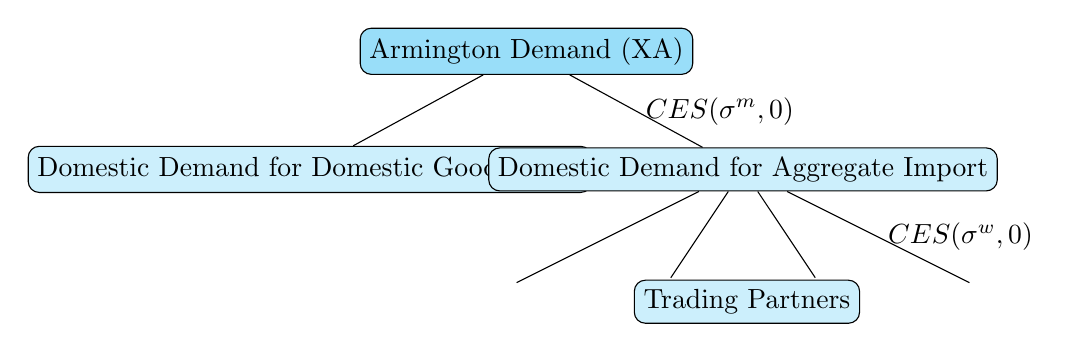
\begin{tikzpicture}

\tikzset{
    level 1/.style={sibling distance=5.5cm},
    level 2/.style={sibling distance=2cm}
}
\node[draw, fill=cyan!40, rounded corners] {\normalsize Armington Demand (XA)}
    child {node[draw, fill=cyan!20, rounded corners] {Domestic Demand for Domestic Goods (XD)}}
    child{node[draw, fill=cyan!20, rounded corners] {Domestic Demand for Aggregate Import}
        child{node { }}
        child{node { }}
        child{node { }}
        child {node { } edge from parent node[right] {$CES(\sigma^w, 0)$}}
    edge from parent node[right] {$CES(\sigma^m, 0)$}
    };
    \path (2.8,-2.9) node[below][draw, fill=cyan!20, rounded corners] {Trading Partners};
\end{tikzpicture}
\end{scriptsize}
\end{center}

\textit{Note(s):}

\begin{footnotesize}
1. \hspace{10pt} The base SAM includes a single trading partner with CALIFORNIA, though the specification of import demand uses the multiple nesting approach in order to provide flexibility for the future as trade data is developed further. Import demand is modeled as a nested CES structure. Agents first choose the optimal level of demand for the so-called Armington good (XA). In a second stage, agents decompose the Armington aggregate good into demand for the domestically produced commodity (XD), and an aggregate import bundle (XM). At the third and final stage, agents choose the optimal quantities of imports from each trading partner. Import prices and tariffs are specific to each of the trading partners.

\end{footnotesize}

\newpage

\begin{center}

Figure 3: \textbf{Output Supply (CET) Nesting}

\vspace{20pt}
\begin{scriptsize}
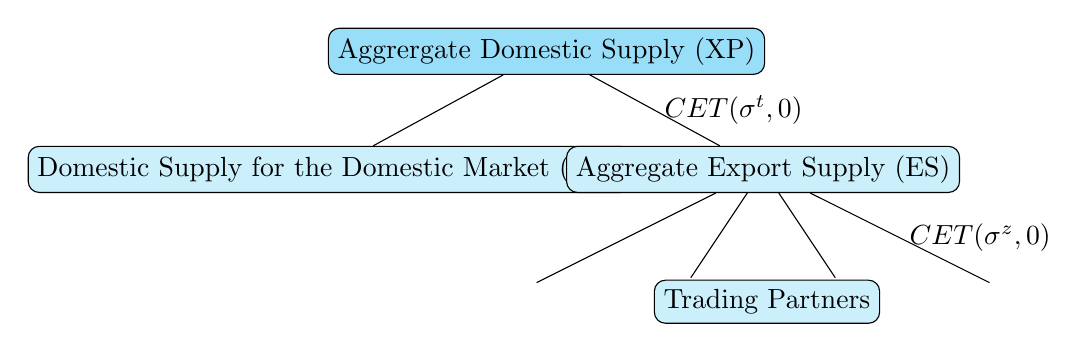
\begin{tikzpicture}

\tikzset{
    level 1/.style={sibling distance=5.5cm},
    level 2/.style={sibling distance=2cm}
}
\node[draw, fill=cyan!40, rounded corners] {\normalsize Aggrergate Domestic Supply (XP)}
    child {node[draw, fill=cyan!20, rounded corners] {Domestic Supply for the Domestic Market (XD)}}
    child{node[draw, fill=cyan!20, rounded corners] {Aggregate Export Supply (ES)}
        child{node { }}
        child{node { }}
        child{node { }}
        child {node { } edge from parent node[right] {$CET(\sigma^z, 0)$}}
    edge from parent node[right] {$CET(\sigma^t, 0)$}
    };
    \path (2.8,-2.9) node[below][draw, fill=cyan!20, rounded corners] {Trading Partners};
\end{tikzpicture}
\end{scriptsize}
\end{center}

\textit{Note(s):}

\begin{footnotesize}
1. \hspace{10pt} The market for domestic output is modeled as a nested CET structure (similar to the note above, the current version of the CALIFORNIA data only concerns a single trading partner). Producers first choose the optimal level of output (XP)\footnote{Note that in a perfectly competitive framework, output is determined by equilibrium conditions, and is not a producer decision.}. In a second stage, producers choose the optimal mix of goods supplied to the domestic market (XD), and an aggregate export supply (ES). At the third and final stage, producers choose the optimal mix of exports to each of the individual trading partners. The export price of each trading partner is region-specific. Under the small-country assumption, the export price is fixed (in out of state currency terms), otherwize, each trading partner has a downward sloping demand curve, and the export price is determined endogenously through an equilibrium condition.


\end{footnotesize}

\newpage
\section*{Appendix 2 - Data Structure for the BEAR Model}
\addcontentsline{toc}{section}{Appendix 2 - Data Structure for the BEAR Model}

The BEAR model is calibrated to a 2022 Social Accounting Matrix for the California economy. This table is based on an extensive synthesis of data from diverse official and independent sources. While the California 2022 SAM is fully documented elsewhere, we summarize the main dimensions of the data in this appendix as they pertain to the BEAR model's structure. The dimensionality of the overall SAM is described in Table A2.1, while component structures used in the BEAR model are discussed individually.

\textbf{Table A2.1: Institutional Structure of the 2022 California SAM}


\framebox[\textwidth][l]{%
  \begin{minipage}{\textwidth}
124 production activities\\
124 commodities (includes trade and transport margins)\\
27 factors of production\\
22 labor categories (skilled and unskilled)\\
\phantomsection{\hspace{10pt}}2 Capital goods (by vintage)\\
\phantomsection{\hspace{10pt}}Land\\
\phantomsection{\hspace{10pt}}Water\\
\phantomsection{\hspace{10pt}}Energy\\
7 Household types, defined by income tax bracket\\
Enterprises\\
Federal Government (7 fiscal accounts)\\
State Government (27 fiscal accounts)\\
Local Government (11 fiscal accounts)\\
Consolidated capital account\\
External Trade Accounts\\
\phantomsection{\hspace{10pt}}Rest of United States\\
\phantomsection{\hspace{10pt}}Rest of the World\\
\end{minipage}}


\newpage
\textbf{Table A2.2: Sector Aggregation}\\[5pt]
\begin{center}
\begin{footnotesize}
\begin{tabular}{|c|c|c|}
\hline & Label & Description \\
\hline 1 & A01 Agric & Agriculture \\
\hline 2 & A02Cattle & Cattle and Feedlots \\
\hline 3 & A03Dairy & Dairy Cattle and Milk Production \\
\hline 4 & A04Forest & Forestry, Fishery, Mining, Quarrying \\
\hline 5 & A05OilGas & Oil and Gas Extraction \\
\hline 6 & A060thPrim & Other Primary Products \\
\hline 7 & A07DistElec & Generation and Distribution of Electricity \\
\hline 8 & A08DistGas & Natural Gas Distribution \\
\hline 9 & A09DistOth & Water, Sewage, Steam \\
\hline 10 & A10ConRes & Residential Construction \\
\hline 11 & A11ConNRes & Non-Residential Construction \\
\hline 12 & A12Constr & Construction \\
\hline 13 & A13FoodPrc & Food Processing \\
\hline 14 & A14TxtAprl & Textiles and Apparel \\
\hline 15 & A15WoodPlp & Wood, Pulp, and Paper \\
\hline 16 & A16PapPrnt & Printing and Publishing \\
\hline 17 & A17OilRef & Oil Refining \\
\hline 18 & A18Chemicl & Chemicals \\
\hline 19 & A19Pharma & Pharmaceutical Manufacturing \\
\hline 20 & A20Cement & Cement \\
\hline 21 & A21Metal & Metal Manufacture and Fabrication \\
\hline 22 & A22Aluminm & Aluminum \\
\hline 23 & A23Machnry & General Machinery \\
\hline 24 & A24AirCon & Air Conditioning and Refrigeration \\
\hline 25 & A25SemiCon & Semi-conductor and Other Computer Manufacturing \\
\hline 26 & A26ElecApp & Electrical Appliances \\
\hline 27 & A27Autos & Automobiles and Light Trucks \\
\hline 28 & A280thVeh & Vehicle Manufacturing \\
\hline 29 & A29AeroMfg & Aeroplane and Aerospace Manufacturing \\
\hline 30 & A30Othind & Other Industry \\
\hline 31 & A31WhiTrad & Wholesale Trade \\
\hline 32 & A32RetVeh & Retail Vehicle Sales and Service \\
\hline 33 & A33AirTrns & Air Transport Services \\
\hline 34 & A34GndTrns & Ground Transport Services \\
\hline 35 & A35WatTrns & Water Transport Services \\
\hline 36 & A36TrkTrns & Truck Transport Services \\
\hline 37 & A37PubTrns & Public Transport Services \\
\hline 38 & A38RetAppl & Retail Electronics \\
\hline 39 & A39RetGen & Retail General Merchandise \\
\hline 40 & A40InfCom & Information and Communication Services \\
\hline 41 & A41FinServ & Financial Services \\
\hline 42 & A42OthProf & Other Professional Services \\
\hline 43 & A43BusServ & Business Services \\
\hline 44 & A44WstServ & Waste Services \\
\hline 45 & A45LandFill & Landfill Services \\
\hline 46 & A46Educatn & Educational Services \\
\hline 47 & A47Medicin & Medical Services \\
\hline 48 & A48Recratn & Recreation Services \\
\hline 49 & A49HotRest & Hotel and Restaurant Services \\
\hline 50 & A500thPrSv & Other Private Services \\
\hline
\end{tabular}
\end{footnotesize}
\end{center}

\newpage

In addition to detailed information on sectoral structure of production, demand, and trade, we detail income and expenditure accounts for a variety of households to better capture distributional impacts of policy. Using data sources that combine California Department of Finance information with household survey and input-output data, we track households in seven tax brackets.

\begin{center}
\begin{small}
\textbf{Table A2.2: California Households and Population by Income Tax Bracket (California Department of Finance: 2006, millions of people)}\\[10pt]
\begin{tabular}{|c|c|c|c|c|c|c|}
\hline & & Households & Cumulative & Population & Cumulative & Percent \\
\hline 1 &  $<$ \$12k & 1.220 & 1.340 & 3.575 & 3.926 & 9.752 \\
\hline 2 & \$12-28k & 2.360 & 3.580 & 6.915 & 10.489 & 18.86 \\
\hline 3 & \$28-40k & 1.650 & 5.230 & 4.835 & 15.324 & 13.19 \\
\hline 4 & \$40-60k & 2.110 & 7.340 & 6.182 & 21.506 & 16.87 \\
\hline 5 & \$60-80k & 1.650 & 8.990 & 4.835 & 26.341 & 13.19 \\
\hline 6 & \$80-200k & 3.140 & 12.130 & 9.200 & 35.541 & 25.10 \\
\hline 7 & \$200k+ & 0.380 & 12.510 & 1.113 & 36.654 & 3.04 \\
\hline & Total & 12.510 & & 36.654 & & 100 \\
\hline
\end{tabular}
\end{small}
\end{center}

\newpage

\textbf{References}\\[20pt]
\addcontentsline{toc}{section}{References}

Abler, D. G., Rodriguez, A. G. and Shortle, J. S. (1999) Parameter uncertainty in CGE modeling of the environmental impacts of economic policies, Environmental and Resource Economics, 14, 75–94.\\
Armington, Paul (1969), “A Theory of Demand for Products Distinguished by Place of Production”,  IMF Staff Papers, vol. 16, pp. 159-178.\\
Ballard, C.L., D. Fullerton, J.B. Shoven, and J. Whalley (1985), A General Equilibrium Model for Tax Policy Evaluation, University of Chicago Press, Chicago.\\
Belgodere, Antoine, Charles Vellutini (2011) Identifying key elasticities in a CGE model: a Monte Carlo approach, Applied Economics Letters, 18:17, 1619-1622\\
Belousov, S. L. (1962), ”Tables of normalized associated Legendre polynomials”, Mathematical tables series Vol. 18, Pergamon Press \\
Borenstein, S. (2006, July). Customer risk from real-time retail electricity pricing: bill volatility and hedge ability, University of California Energy Institute, working paper CSEM WP 155. [Available Online] http://www. ucei.org.\\
Borenstein, S. (2006, July). Wealth transfer among large customers from implementing real-time retail electricity pricing, University of California Energy Institute, working paper CSEM WP 156. [Available Online] http://www.ucei.org.Deaton, Angus and John Muellbauer (1980), Economics and Consumer Behavior, Cambridge University Press, Cambridge, UK.\\
Dessus, Sébastien, David Roland-Holst, and Dominique van der Mensbrugghe (1994), “Input-Based Pollution Estimates for Environmental Assessment in Developing Countries”, Technical Papers, No. 101, OECD Development Centre, Paris, October.\\
DeVuyst, E.A. and P.V. Preckel (1997), ”Sensitivity Analysis Revisited: A Quadrature-Based Approach”, Journal of Policy Modeling 19, 175-185. \\
European Union (2008) Guide to Cost Benefit Analysis of Investment Projects. Structural Funds, Cohesion Fund and Instrument for Pre-Accession. July 2008. EUROPEAN COMMISSION. Directorate General Regional Policy. \\
Fullerton, D. (1983), “Transition Losses of Partially Mobile Industry-specific Capital”, Quarterly Journal of Economics, February, pp. 107-125. \\
Greenwood,R.E.andJ.J.Miller(1948),”Zeros of the Hermite polynomials and weights for Gauss’ mechanical quadrature formula”, Bull. Amer. Math. Soc. 54 (8), 765-769  \\
Harrison, Glenn, Richard Jones, Larry Kimbell and Randall Wigle. “How Robust Is Applied General Equilibrium Analysis?”, Journal of Policy Modeling, 15(1): 99-115. \\
Hermeling, C., A. Loschel, T. Minnel (2013) “A new robustness analysis for climate policy evaluations: A CGE application for the EU 2020 targets,” Energy Policy, 55, 27-35. \\
Howe, H. (1975), “Development of the Extended Linear Expenditure System from Simple Savings Assumptions”, European Economic Review, Volume 6, pp. 305-310. \\
Leamer, E. (1985), ”Sensitivity Analyses would Help”, American Economic Review 75 (3), 308-313  \\
Lee, F.N.  M. Lin and A.M. Breipohl, Evaluation of the variance of production cost using a stochastic outage capacity state model, IEEE Trans. Power Syst., 5 (4) (1990) 1061-1067. \\
Lluch, C. (1973), “The Extended Linear Expenditure System”, European Economic Review, Volume 4, pp.21-32.\\
Martin, Paul, David Wheeler, Mala Hettige, and Ralph Stengren (1991), “The Industrial Pollution Projection System: Concept, Initial Development, and Critical Assessment”, Mimes, The World Bank, Washington, D.C. \\
Mazumdar, M.  and A. Kapoor, Stochastic models for power generation system production costs, Eleetr. Power Syst. Res., 35 (1995) 93 -100. \\
Ryan S.M.  and M. Mazumdar, Effect of frequency and duration of generating unit outages on distribution of system production costs, IEEE Trans. Power Syst., 5 (1)(1990) 191--197. \\
S.M. Ryan and M. Mazumdar, Chronological influences on the variance of electric power production costs, Oper. Res. Suppl. 40 (2) (1990) $284 $292. \\
Scully A.  et al. (1992) Using a semi-guided Monte Carlo method for faster simulation of forced outages of generating units, 1EEE Trans. Power Syst., 7 (3) (1992) 1313 1321. \\
Seko K (1987) Seasonal variation of altitudinal dependence of precipitation in Langtang Valley, Nepal Himalayas. Bull Glacier Res 5:41–47 \\
Spezia, Carl J. (2009) “Monte Carlo Analysis of Real-Time Electricity Pricing for Industrial Loads,” Journal of Industrial Technology. Volume 25, Number 3, July-September. \\
Vose, David. 1996. Quantitative Risk Analysis: A Guide to Monte Carlo Simulation Modelling, Wiley, Chichester.


\end{document}